\documentclass[conference]{IEEEtran}
\usepackage{float}
\IEEEoverridecommandlockouts
\usepackage{cite}
\usepackage{placeins}
\usepackage{amsmath,amssymb,amsfonts}
\usepackage{algorithmic}
\usepackage{graphicx}
\graphicspath{{Image/}}
\usepackage[hidelinks]{hyperref}
\usepackage{textcomp}
\usepackage{xcolor}
\usepackage{url}
\usepackage{booktabs}
\usepackage[utf8]{inputenc}
\usepackage[T1]{fontenc}
\usepackage[spanish,es-noshorthands]{babel}
\usepackage{tabularx}
\usepackage{multirow}
\usepackage{enumitem}

\def\BibTeX{{\rm B\kern-.05em{\sc i\kern-.025em b}\kern-.08em
    T\kern-.1667em\lower.7ex\hbox{E}\kern-.125emX}}

\newcommand{\metric}[1]{\textbf{#1}}
\newcommand{\code}[1]{\texttt{#1}}

\begin{document}

\title{Modelos Predictivos de Machine Learning para la Clasificación de Diabetes en el Dataset Pima Indians}

\author{
\IEEEauthorblockN{1\textsuperscript{st} Ronal Mora-Aybar}
\IEEEauthorblockA{\textit{Facultad de Ingeniería - ITIS} \\
\textit{Universidad ESAN}\\
Lima, Perú \\
22200234@ue.edu.pe}
\and
\IEEEauthorblockN{2\textsuperscript{nd} Andres Quiliche}
\IEEEauthorblockA{\textit{Facultad de Ingeniería - ITIS} \\
\textit{Universidad ESAN}\\
Lima, Perú \\
22200144@ue.edu.pe}
\and
\IEEEauthorblockN{3\textsuperscript{rd} Angel Aguilar}
\IEEEauthorblockA{\textit{Facultad de Ingeniería - ITIS} \\
\textit{Universidad ESAN}\\
Lima, Perú \\
22200133@ue.edu.pe}
}
\maketitle

\begin{abstract}
La diabetes crece de forma sostenida en el Perú y presiona a un sistema de salud con capacidad limitada para confirmar y dar seguimiento a los casos. Frente a ese problema, este informe construye y evalúa un pipeline completo de minería de datos para clasificar diabetes a partir del conjunto Pima Indians Diabetes. El flujo sigue una secuencia ordenada: primero se explora y depura la información ---tratamiento de valores faltantes, control de outliers, transformación y escalado robusto---; luego se comparan cinco modelos base y cinco de ensamble, además de un modelo de stacking, bajo un mismo protocolo de validación; y, por último, se interpretan las predicciones con SHAP. Para evitar la fuga de información, se retiraron 6 coincidencias exactas entre las particiones, con lo que el entrenamiento quedó en 2\,460 registros y la prueba en 302. El mejor modelo fue Bagging de árboles (ROC AUC = 0.8937, F1 = 0.7222, accuracy = 0.8344 en test), que superó por un margen mínimo al Stacking Top-3 (ROC AUC = 0.8889). El análisis con SHAP muestra que \code{Glucose} es, con diferencia, la variable más influyente ---seguida de \code{BMI}, \code{Age} y \code{DiabetesPedigreeFunction}--- y que su efecto es clínicamente coherente: a mayor valor, mayor probabilidad predicha de diabetes. A partir de ese resultado, se propone emplear el score del modelo como mecanismo de priorización ---ordenar a los pacientes por riesgo para acelerar su confirmación diagnóstica y seguimiento--- y no como sustituto de la decisión clínica.
\end{abstract}

\begin{IEEEkeywords}
diabetes, minería de datos, machine learning, clasificación, Bagging, XGBoost, SHAP, Pima Indians, ROC AUC.
\end{IEEEkeywords}

\section{Introducción}

La diabetes mellitus es una enfermedad crónica de alta relevancia sanitaria por su asociación con complicaciones cardiovasculares, renales, neurológicas y visuales, y constituye una de las principales enfermedades no transmisibles a nivel global \cite{idf2021,who2021}. En el Perú, la diabetes muestra una trayectoria ascendente: la prevalencia autorreportada en personas de 15 años a más pasó de 3.9\% en 2019 a 4.5\% en 2020, 4.9\% en 2021 y 5.5\% en 2023. Este cambio equivale a un aumento de 1.6 puntos porcentuales y a un crecimiento relativo aproximado de 41\% frente a 2019. El último dato nacional explícito revisado corresponde a ENDES 2023, resumido por MINSA como cerca de 1.3 millones de peruanos mayores de 15 años viviendo con diabetes \cite{minsa2024,inei2023}.

La carga no es únicamente epidemiológica. El CDC Perú reportó 54\,986 casos registrados entre enero de 2023 y junio de 2024 y advirtió subregistro; para 2025 la red de notificación incluía 1\,600 establecimientos, de los cuales 1\,440 correspondían al primer nivel de atención \cite{cdc2024,cdc2025}. Esto evidencia un sistema en expansión, pero todavía con brechas de registro, confirmación diagnóstica y seguimiento.

En este contexto, los modelos de machine learning pueden apoyar la priorización de pacientes con mayor probabilidad de diabetes, especialmente cuando se usan como herramientas de apoyo a la decisión clínica y no como sustitutos del diagnóstico médico. El reto técnico consiste en construir un flujo reproducible que evite fuga de información, trate correctamente los valores faltantes y permita comparar modelos con métricas adecuadas. El reto aplicado consiste en convertir el resultado del modelo en una acción útil: priorizar al paciente con mayor riesgo para confirmación rápida mediante glucemia en ayunas, HbA1c o prueba de tolerancia oral a la glucosa. Estudios previos sobre diabetes han mostrado el valor de modelos de clasificación y minería de datos para este tipo de problema \cite{kavakiotis2017,sisodia2018}.

El objetivo del proyecto es desarrollar y evaluar un pipeline de minería de datos para predecir la variable binaria \code{Outcome}, donde 0 representa ausencia de diabetes y 1 presencia de diabetes, usando variables clínicas y antropométricas del dataset Pima Indians. El código completo y los recursos del proyecto están disponibles públicamente en el repositorio del proyecto\footnote{\url{https://github.com/23-Andres-QC/ProyectoFinalMineria}}.

\section{Contexto Peruano}

La carga de diabetes en el Perú no se distribuye de manera uniforme y ejerce una presión creciente sobre el sistema de salud. La prevalencia es mayor en la Costa (6.0\% en 2022) que en la Selva (4.5\%) y la Sierra (3.0\%), y se concentra sobre todo en los adultos mayores, entre quienes alcanzó 14.0\% en 2023 y 2024. A esta mayor demanda se suma una red de vigilancia epidemiológica todavía en expansión, lo que tensiona consultas, laboratorios y programas de control de enfermedades crónicas \cite{pp0018,inei_adulto_mayor}. La Tabla~\ref{tab:contexto_peru} resume los principales indicadores nacionales revisados.

\begin{table}[H]
\centering
\caption{Métricas de referencia sobre diabetes en Perú}
\label{tab:contexto_peru}
\scriptsize
\begin{tabularx}{\columnwidth}{@{}lX@{}}
\toprule
\textbf{Indicador} & \textbf{Hallazgo resumido} \\
\midrule
Prevalencia 15+ & 3.9\% (2019), 4.5\% (2020), 4.9\% (2021), 5.5\% (2023). \\
Personas afectadas & Aproximadamente 1.3 millones de peruanos mayores de 15 años en 2023. \\
Mortalidad & Diabetes reportada por MINSA como séptima causa de muerte en 2024. \\
Vigilancia & 54\,986 casos registrados entre enero de 2023 y junio de 2024; CDC advierte subregistro. \\
Red notificante & 1\,600 IPRESS en 2025: 1\,440 de primer nivel y 160 hospitales. \\
Adultos mayores & 14.0\% de prevalencia en población de 60 años a más en 2024. \\
Brecha operativa & No existe un promedio nacional público uniforme desde primera consulta hasta diagnóstico confirmado. \\
\bottomrule
\end{tabularx}
\end{table}

\subsection{Métricas Operativas de Referencia}

En la práctica peruana, el diagnóstico se apoya en tres pruebas centrales, cuyos umbrales e implicancias operativas se resumen en la Tabla~\ref{tab:pruebas_operativas}: la glucemia en ayunas es ampliamente disponible pero exige que el paciente llegue en ayunas; la HbA1c no requiere ayuno y puede reducir visitas; y la PTOG de 75 g requiere una permanencia mínima de dos horas. Los tiempos de entrega no suelen ser el cuello de botella: en laboratorios privados, glucosa, HbA1c y PTOG se reportan en menos de 24 horas o en 1 día hábil, y en un hospital público grande los exámenes generales se entregan en 1 día hábil \cite{multilab_glucosa,multilab_hba1c,loayza2025}. El problema, por tanto, está menos en la velocidad del laboratorio y más en el circuito: el ayuno, las visitas repetidas y la continuidad del seguimiento.

\begin{table}[H]
\centering
\caption{Pruebas diagnósticas y tiempos operativos de referencia}
\label{tab:pruebas_operativas}
\scriptsize
\begin{tabularx}{\columnwidth}{@{}lXX@{}}
\toprule
\textbf{Prueba} & \textbf{Umbral de diabetes} & \textbf{Implicancia operativa} \\
\midrule
Glucemia en ayunas & $\geq 126$ mg/dL & Bajo costo y alta disponibilidad; puede requerir nueva visita si el paciente no llegó en ayunas. \\
HbA1c & $\geq 6.5\%$ & No requiere ayuno; útil para acortar el circuito diagnóstico si está disponible. \\
PTOG 75 g & $\geq 200$ mg/dL a las 2 h & Más lenta; requiere al menos 2 horas de permanencia. \\
\bottomrule
\end{tabularx}
\end{table}

Para consulta externa, no se encontró un indicador nacional reciente de pacientes por día específicamente en consulta de diabetes. Sin embargo, la programación hospitalaria del MINSA usa turnos de 4 horas y varios documentos de gestión emplean productividades de 4 a 5 consultas por hora. Con esa referencia, un consultorio puede atender aproximadamente 16--20 pacientes por turno, o 32--40 si opera en doble turno. Esta restricción de capacidad refuerza la necesidad de priorizar mejor a los pacientes con mayor riesgo.

\subsection{Rol Propuesto del Modelo}

El modelo desarrollado no pretende diagnosticar de forma autónoma, sino actuar como un \textbf{filtro de priorización}: ordenar a los pacientes por probabilidad estimada de diabetes para acelerar la confirmación de los casos de mayor riesgo. Conviene precisar un límite del enfoque desde ahora: el score se calcula a partir de las variables de entrada del modelo ---incluida \code{Glucose}---, de modo que no decide si solicitar una primera prueba, sino que ordena la confirmación diagnóstica y el seguimiento una vez disponible una medición inicial. Bajo esa premisa, el valor del modelo está en reducir esperas, visitas innecesarias y pérdidas de seguimiento; la forma concreta de insertarlo en el circuito de atención se detalla más adelante (Sección~\ref{sec:impacto}).

\section{Revisión de Literatura}

La literatura sobre predicción de diabetes con machine learning suele trabajar con datos tabulares clínicos, donde las variables antropométricas, bioquímicas y demográficas permiten estimar riesgo mediante clasificadores supervisados. Revisiones previas han mostrado que algoritmos como SVM, redes neuronales, Naive Bayes, árboles de decisión y métodos de ensamble han sido ampliamente usados en problemas de diabetes \cite{kavakiotis2017,sisodia2018}.

En datos tabulares, los métodos de ensamble suelen ser competitivos porque combinan múltiples modelos débiles o moderados para reducir varianza o sesgo. Bagging promedia árboles entrenados sobre muestras bootstrap, mientras que boosting entrena modelos secuenciales que corrigen errores anteriores. Implementaciones como XGBoost y LightGBM han destacado por su eficiencia y regularización en problemas de clasificación \cite{chen2016,ke2017}.

No obstante, el rendimiento predictivo no es suficiente en salud. Un modelo de apoyo clínico debe ser interpretable, trazable y compatible con decisiones operativas. Por ello, SHAP se usa como técnica de explicación para estimar la contribución de cada variable a las predicciones del modelo \cite{lundberg2017}. En este proyecto, SHAP permite verificar si los predictores más influyentes coinciden con la evidencia clínica y con los hallazgos estadísticos del análisis exploratorio.

\section{Metodología}
\label{sec:metodologia}

El estudio sigue la metodología de Box-Jenkins \cite{box2015,hyndman2021} para modelar la serie: transformación, prueba de estacionariedad, identificación, estimación, validación de residuos y pronóstico. Sobre esa base se construye un SARIMAX con dos variables exógenas y se compara con Prophet, modelos de machine learning, AutoML, redes neuronales recurrentes, un Transformer entrenado desde cero y Transformers preentrenados. Todos se evalúan con el mismo protocolo de pronóstico. Las subsecciones describen, en orden, la recolección de los datos, su preparación y las técnicas de análisis.

\subsection{Recolección de los Datos}

Los datos se descargaron con código directamente de sus fuentes oficiales. Del Banco Central de Reserva del Perú (BCRP), mediante la API de BCRPData \cite{bcrpdata}, se obtuvieron el índice del PBI del sector Electricidad y Agua (2007 = 100), su variación porcentual interanual y el precio internacional del cobre. Del Instituto Geofísico del Perú (IGP) se obtuvo el archivo oficial del Índice Costero El Niño (ICEN) que publica el ENFEN \cite{igp_icen,takahashi2015}. Todas las series son mensuales. La Tabla~\ref{tab:series} resume el rol de cada una.

\begin{table}[H]
\centering
\caption{Series utilizadas, fuente y transformación}
\label{tab:series}
\scriptsize
\begin{tabularx}{\columnwidth}{@{}lXl@{}}
\toprule
\textbf{Rol} & \textbf{Serie (fuente, código)} & \textbf{Transformación} \\
\midrule
Objetivo $I_t$ & Índice del PBI Electricidad y Agua, 2007 = 100 (BCRP, \code{PN01765AM}) & $z_t = 100\ln I_t$ \\
Control & Variación \% interanual del sector (BCRP, \code{PN01723AM}) & Ninguna \\
Exógena $x_{1t}$ & Precio del cobre LME, \textcent US\$/lb (BCRP, \code{PN01652XM}) & $100\ln x_{1t}$ \\
Exógena $x_{2t}$ & ICEN, anomalía en \textdegree C (ENFEN/IGP) & Ninguna \\
\bottomrule
\end{tabularx}
\end{table}

Se trabaja con el índice en niveles y no con su variación porcentual porque el logaritmo solo está definido para valores positivos: el índice siempre lo es, mientras que la variación toma valores negativos. La variación interanual oficial (\code{PN01723AM}) se usa como control: la variación calculada a partir del índice coincide con ella (diferencia máxima de $5.2\times10^{-14}$) y es la cifra contra la que se evalúan los pronósticos. El periodo de descarga termina en julio de 2026 y queda fijo para que los resultados sean reproducibles. Aun así, el BCRP revisa sus cifras y los últimos meses del ICEN son provisionales (es una media móvil centrada de tres meses), por lo que una nueva descarga puede dar valores algo distintos.

El índice está disponible desde enero de 1994, el cobre desde enero de 2000 y el ICEN desde enero de 1950. La muestra de análisis va de enero de 2002 a julio de 2026 (295 observaciones mensuales, sin faltantes). Empieza en 2002 para que puedan probarse rezagos de hasta 12 meses en las exógenas con datos de cobre disponibles.

Las variables exógenas se eligieron con tres criterios. Primero, debían ser \textbf{externas al sector}: el INEI calcula el PBI de Electricidad y Agua con los volúmenes físicos de producción de electricidad, gas y agua \cite{inei2017}, de modo que se descartaron otros sectores del PBI, la demanda interna y la producción eléctrica en GWh, que forman parte del cálculo. Segundo, debían tener un \textbf{canal causal documentado}. La gran minería es el mayor consumidor de electricidad del país \cite{bcrp_moneda198}, y un cobre caro impulsa su producción y sus ampliaciones. El Niño Costero, por su parte, trae lluvias y huaicos que dañan captaciones y plantas de agua y altera la hidrología de las centrales hidroeléctricas \cite{inei2017,takahashi2015}. Tercero, debían contar con \textbf{datos mensuales oficiales desde 2000}. También se evaluaron el tipo de cambio, el IPC, las expectativas empresariales y la temperatura de Lima, pero se descartaron porque su canal hacia el sector es más indirecto o porque se superponen con el ICEN. La Fig.~\ref{fig:serie_exogenas} muestra la serie y las dos exógenas.

\begin{figure}[H]
  \centering
  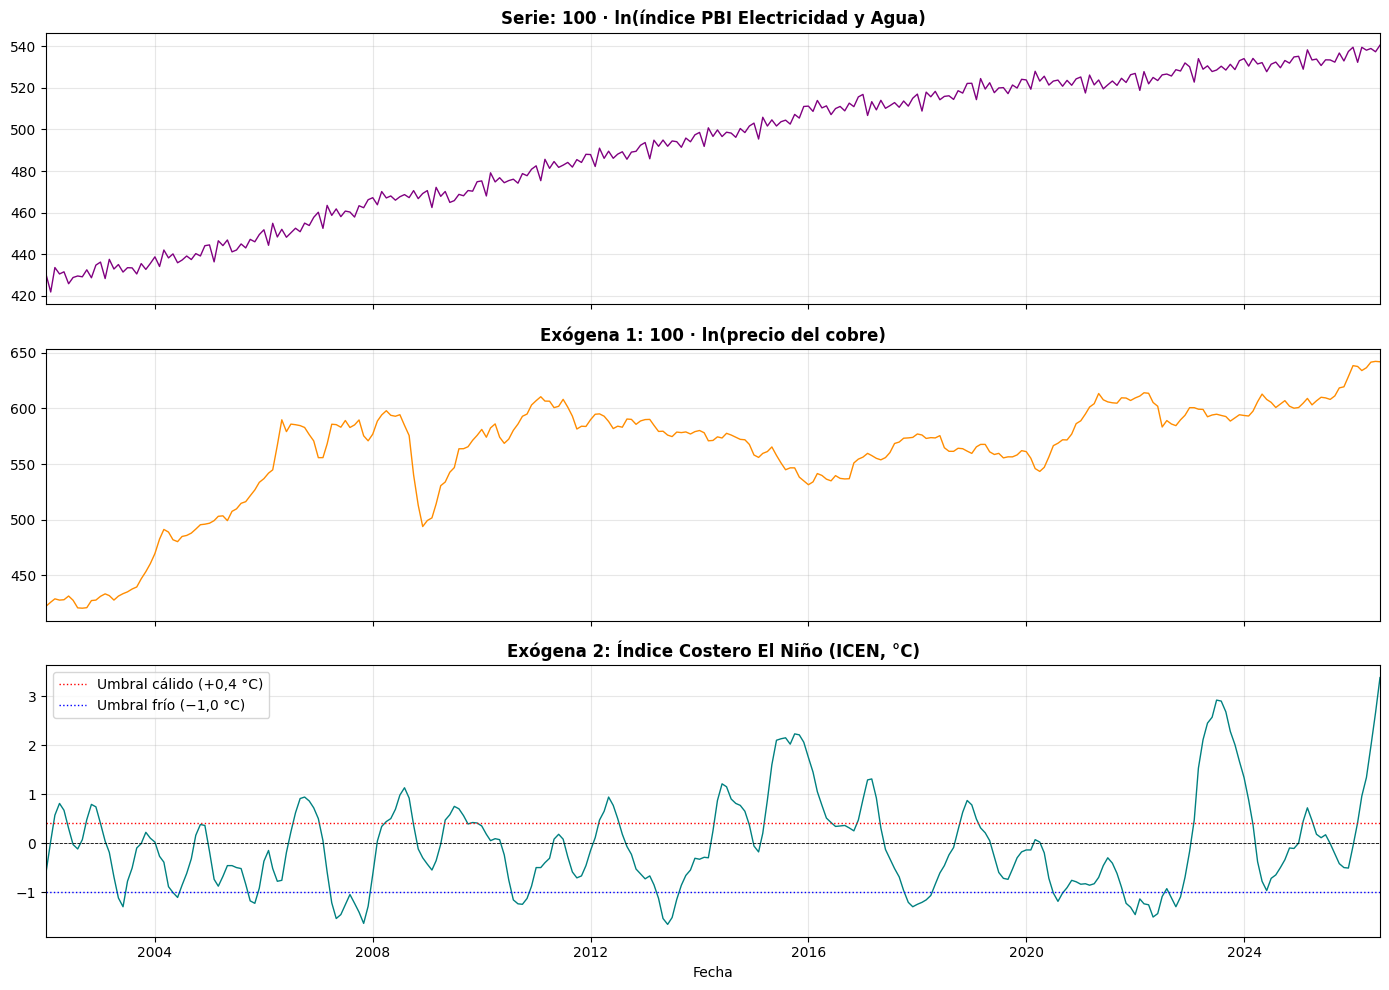
\includegraphics[width=\columnwidth]{m02_serie_exogenas.png}
  \caption{Serie en logaritmos ($100\ln I_t$), precio del cobre en logaritmos e ICEN, enero 2002 -- julio 2026.}
  \label{fig:serie_exogenas}
\end{figure}

\subsection{Preparación y Transformación de la Serie}

\textbf{Tratamiento de la pandemia.} Los meses de marzo de 2020 a junio de 2021 (confinamiento y rebote) son atípicos y se reemplazaron. Como se modela el índice en niveles, la imputación debe empalmar con los datos reales a ambos lados del tramo. El procedimiento, en logaritmos, fue: 1) estimar la estacionalidad típica de cada mes con los datos de 1994--2019 mediante una descomposición aditiva; 2) restarla a la serie; 3) interpolar linealmente el nivel desestacionalizado entre febrero de 2020 y julio de 2021; y 4) volver a sumar la estacionalidad de cada mes. Las exógenas no se imputaron, porque son fenómenos externos y sus valores durante la pandemia son reales.

\textbf{Transformación logarítmica.} Antes de decidir la diferenciación, la serie se transformó con $z_t = 100\ln I_t$. El logaritmo estabiliza la varianza: en niveles, la dispersión de los meses dentro de cada año crece con el índice (la correlación entre nivel y dispersión anual es 0.86), mientras que en logaritmos esa correlación baja a $-0.33$ y la estacionalidad pasa de multiplicativa a aditiva. Además, las diferencias de $z_t$ se leen como tasas de crecimiento en puntos porcentuales y, al deshacer la transformación con $I_t = e^{z_t/100}$, el pronóstico del índice nunca es negativo. El cobre recibió la misma transformación, de modo que su coeficiente es una elasticidad. El ICEN no se transformó porque toma valores negativos (Fig.~\ref{fig:imputacion_log}).

\begin{figure}[H]
  \centering
  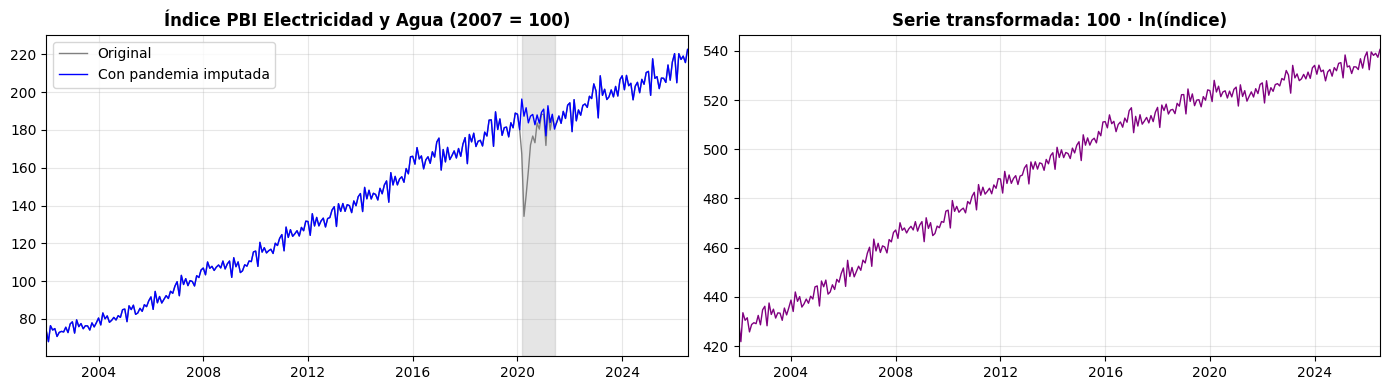
\includegraphics[width=\columnwidth]{m01_imputacion_log.png}
  \caption{Índice original y con la pandemia imputada (izquierda) y serie transformada $100\ln I_t$ (derecha). La franja gris marca marzo 2020 -- junio 2021.}
  \label{fig:imputacion_log}
\end{figure}

\textbf{Análisis descriptivo.} Se calcularon estadísticos de posición y forma (media, desviación estándar, asimetría y curtosis), cuartiles y deciles. La regla de Tukey ($Q_1 - 1.5\,\mathrm{IQR}$, $Q_3 + 1.5\,\mathrm{IQR}$) se aplicó a la variación interanual y no al índice: en una serie con tendencia, los cuantiles del nivel separan épocas y no meses normales de anormales. El crecimiento mensual se resumió por cuartiles para cada mes del calendario, con el fin de caracterizar la estacionalidad.

\subsection{Estacionariedad e Identificación del Modelo}

Con los datos de entrenamiento se evaluaron cuatro versiones de $z_t$: sin diferenciar, con primera diferencia ($d=1$), con diferencia estacional ($D=1$, $s=12$) y con ambas. Una versión se consideró estacionaria cuando cumplía tres criterios: la prueba ADF rechaza la raíz unitaria ($p<0.05$) \cite{dickey1979}, la prueba KPSS no rechaza la estacionariedad ($p\geq0.05$) \cite{kpss1992} y la autocorrelación en el rezago 12 es menor a 0.5. Este último es un criterio práctico para detectar una estacionalidad no estacionaria que el ADF no capta. Se eligió la versión con menos diferencias que cumple los tres criterios: $d=1$ y $D=1$. La FAC y la FACP de la serie diferenciada (Fig.~\ref{fig:fac_facp}) muestran picos negativos aislados en los rezagos 1 y 12, lo que apunta a un MA(1) regular y un MA(1) estacional, es decir, al ``modelo de aerolínea'' de Box y Jenkins.

\begin{figure}[H]
  \centering
  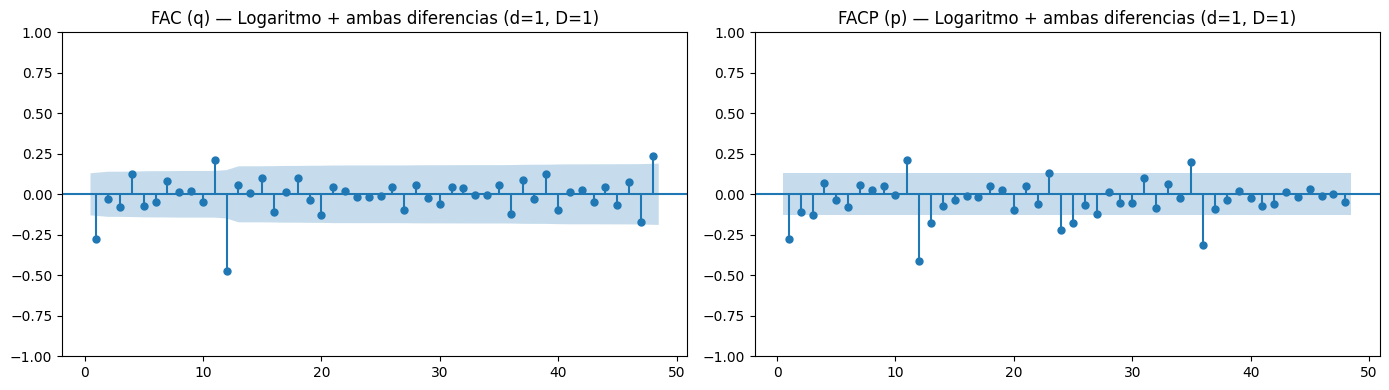
\includegraphics[width=\columnwidth]{m04_fac_facp_diferenciada.png}
  \caption{FAC y FACP de $z_t$ con $d=1$ y $D=1$ (datos de entrenamiento).}
  \label{fig:fac_facp}
\end{figure}

Las diferencias elegidas se incluyen dentro del modelo SARIMA$(p,d,q)(P,D,Q)_{12}$:
\begin{equation}
\phi_p(B)\,\Phi_P(B^{12})\,(1-B)^{d}(1-B^{12})^{D} z_t = \theta_q(B)\,\Theta_Q(B^{12})\,\varepsilon_t,
\label{eq:sarima}
\end{equation}
donde $B$ es el operador de rezago y $\varepsilon_t$ es ruido blanco. Como $d+D=2$, el modelo no lleva constante. Se estimaron por máxima verosimilitud todas las combinaciones con $p,q\in\{0,\dots,3\}$ y $P,Q\in\{0,1\}$ (con $p+q\leq4$ cuando hay términos estacionales) y se agruparon en cuatro familias: AR, MA y ARMA (con las diferencias, pero sin términos estacionales) y SARIMA. Aparte, se estimó un ARIMA$(p,1,q)$ clásico con deriva, sin diferencia ni términos estacionales, para medir cuánto aporta la parte estacional; su AIC y BIC solo se comparan entre modelos ARIMA. El criterio de selección fue el menor BIC entre los modelos cuyos residuos pasan la prueba de Ljung-Box en los rezagos 12 y 24, con los grados de libertad corregidos por los parámetros estimados \cite{ljungbox1978}. Un modelo con residuos autocorrelacionados se descarta y se vuelve a la identificación.

\subsection{Partición de la Muestra}

El entrenamiento abarca de enero de 2002 a diciembre de 2021 (240 meses, 81\%) y la prueba, de enero de 2022 a julio de 2026 (55 meses, 19\%). La prueba empieza después del tramo imputado de la pandemia, de modo que los modelos se evalúan solo con datos reales. Todas las decisiones (diferencias, órdenes, rezagos de las exógenas, hiperparámetros y arquitecturas) se tomaron con el entrenamiento; la prueba se usó únicamente para la evaluación final.

\subsection{Modelo SARIMAX y Selección de Rezagos}

Al incorporar las exógenas, el modelo pasa a ser un SARIMAX: una regresión cuyos errores siguen el SARIMA identificado,
\begin{equation}
z_t = \beta_1\, 100\ln(\mathrm{cobre}_{t-L_1}) + \beta_2\, \mathrm{ICEN}_{t-L_2} + u_t,
\label{eq:sarimax}
\end{equation}
con $u_t \sim$ SARIMA$(p,d,q)(P,D,Q)_{12}$. El coeficiente $\beta_1$ es una elasticidad (un cobre 10\% más caro cambia el índice en $\approx 10\beta_1$\%) y $\beta_2$, una semielasticidad (cada \textdegree C adicional de ICEN cambia el índice en $\approx \beta_2$\%).

El efecto de las exógenas no tiene por qué ser inmediato: un alza del cobre tarda meses en convertirse en más producción minera, y El Niño afecta la infraestructura con retraso. Por ello se probaron rezagos $L$ de 0 a 12 meses en dos pasos: 1) se calculó la correlación cruzada entre la serie y cada exógena, ambas con las mismas diferencias ($d=1$, $D=1$); y 2) para cada rezago se estimó un SARIMAX con una sola exógena y el orden base, y se eligió el rezago de menor BIC. El resultado fue $L_1=7$ meses para el cobre y $L_2=10$ meses para el ICEN. El rezago tiene, además, una ventaja práctica: los primeros $L$ meses del pronóstico usan valores ya observados de la exógena. El rezago 0 del ICEN no estaría disponible al momento de pronosticar, porque es una media móvil centrada.

Se estimaron tres versiones con el mismo orden: solo cobre, solo ICEN y cobre + ICEN (modelo propuesto). Como las diferencias de BIC entre estas versiones y el SARIMA son menores a 2 puntos (evidencia débil), entre modelos del mismo orden se usó el AIC, el criterio orientado al pronóstico, y se mantuvieron ambas exógenas por su sentido económico.

\subsection{Modelo Prophet}

Como alternativa al enfoque de Box-Jenkins se usó Prophet \cite{taylor2018}, un modelo aditivo que descompone la serie en tendencia, estacionalidad y regresores:
\begin{equation}
z_t = g(t) + s(t) + \boldsymbol{\gamma}^{\top}\mathbf{x}_t + \varepsilon_t,
\label{eq:prophet}
\end{equation}
donde $g(t)$ es una tendencia lineal por tramos con puntos de cambio y $s(t)$ es una estacionalidad anual representada con 6 armónicos de Fourier (sin estacionalidad semanal ni diaria, porque los datos son mensuales). Se ajustó sobre la misma serie $z_t = 100\ln I_t$ en dos versiones: univariada y con los regresores del SARIMAX ($\mathbf{x}_t$: cobre en $t-7$ e ICEN en $t-10$). Los hiperparámetros \code{changepoint\_prior\_scale} $\in\{0.01, 0.05, 0.1, 0.5\}$ y \code{seasonality\_prior\_scale} $\in\{0.1, 1, 10\}$ se eligieron sin mirar la prueba, con una validación interna: se entrena hasta diciembre de 2016 y se mide el RMSE del pronóstico a un mes de enero de 2017 a diciembre de 2019. Como Prophet no tiene parte autorregresiva, en el pronóstico a un mes se reestima cada mes con origen móvil. Los coeficientes de los regresores se compararon con los del SARIMAX.

\subsection{Esquemas de Pronóstico y Métricas de Evaluación}

Cada modelo se estimó solo con el entrenamiento y pronosticó $z_t$, que luego se llevó a la escala del índice con $I_t = e^{z_t/100}$. A partir del índice se calculó la variación interanual, tomando como base el índice real de hace 12 meses, y se comparó con la cifra oficial del BCRP. Se evaluaron dos esquemas:
\begin{itemize}[leftmargin=*]
  \item \textbf{Horizonte completo:} los 55 meses de prueba se pronostican de una sola vez desde diciembre de 2021.
  \item \textbf{A un mes:} cada mes se pronostica el siguiente con el dato real del mes anterior, manteniendo fijos los parámetros del entrenamiento. Es el uso real de un modelo mensual y el escenario común en el que se comparan todos los modelos.
\end{itemize}
En la prueba, los SARIMAX usan los valores observados de las exógenas. A un mes esto no da ventaja, porque con rezagos de 7 y 10 meses esos valores ya se conocen; en el horizonte completo, más allá de esos rezagos, la ventaja frente al SARIMA es optimista. Como referencia se usaron dos modelos ingenuos: el \textbf{ingenuo estacional} (el índice repite el del mismo mes del año anterior) y el \textbf{ingenuo con último crecimiento} (el índice crece al último ritmo interanual conocido).

Las métricas se calcularon sobre el índice: MSE, RMSE y MAE (en puntos del índice) y MAPE. El MAPE es interpretable porque el índice toma valores entre 150 y 230 y nunca se acerca a cero. Se añadieron el RMSE de la variación interanual (en puntos porcentuales), el Índice de Error Compuesto (IEC), que promedia las cuatro métricas normalizadas como $m/(1+m)$, el MASE \cite{hyndman2006} y la U de Theil \cite{theil1966}:
\begin{equation}
\mathrm{MASE} = \frac{\mathrm{MAE}}{\frac{1}{n-12}\sum_{t=13}^{n}\lvert I_t - I_{t-12}\rvert},
\label{eq:mase}
\end{equation}
\begin{equation}
U_2 = \sqrt{\frac{\sum_t \left(\frac{\hat{I}_t - I_t}{I_{t-1}}\right)^2}{\sum_t \left(\frac{I_t - I_{t-1}}{I_{t-1}}\right)^2}},
\label{eq:theil}
\end{equation}
donde el denominador del MASE es el MAE del ingenuo estacional en el entrenamiento. Un MASE o una $U_2$ menores a 1 indican que el modelo supera al ingenuo estacional y al ingenuo ``sin cambio'', respectivamente. La significancia de las diferencias entre dos pronósticos se evaluó con la prueba de Diebold-Mariano sobre el error cuadrático \cite{diebold1995}.

Por último, se verificó que los residuos del modelo propuesto se comporten como ruido blanco: sin autocorrelación (Ljung-Box), con varianza constante (prueba ARCH \cite{engle1982}) y con distribución normal (Jarque-Bera \cite{jarque1980}). Se descartaron los primeros 13 residuos, que corresponden a la inicialización de las diferencias.

\subsection{Modelos de Machine Learning: Boosting y AutoML}

Los árboles de decisión no requieren estacionariedad, pero no extrapolan: solo predicen valores dentro del rango visto en el entrenamiento. En la prueba, el índice supera el máximo del entrenamiento en el 78\% de los meses, por lo que se descartó como objetivo. En su lugar se modeló el crecimiento mensual logarítmico, $r_t = \ln(I_t/I_{t-1})$ (\code{Log\_Return}), y el índice se reconstruyó con $\hat{I}_t = I_{t-1}\,e^{\hat{r}_t}$. Todos los predictores se conocen al cierre del mes $t-1$, para evitar fuga de información (Tabla~\ref{tab:predictores}).

\begin{table}[H]
\centering
\caption{Predictores de los modelos de machine learning}
\label{tab:predictores}
\scriptsize
\begin{tabularx}{\columnwidth}{@{}lX@{}}
\toprule
\textbf{Grupo} & \textbf{Variables} \\
\midrule
Rezagos del objetivo & $r_{t-1},\dots,r_{t-12}$; $r_{t-12}$ recoge la estacionalidad. \\
Cambio del mes anterior & Rendimiento simple y variación absoluta del índice en $t-1$. \\
Medias móviles relativas & $\ln(I_{t-1}/\mathrm{MA}_k)$ para $k=3,6,9$; se usa la versión relativa porque el nivel de la media móvil no extrapola. \\
Calendario & Mes del año. \\
Exógenas & Crecimiento logarítmico del cobre en $t-7$ e ICEN en $t-10$ (los rezagos del SARIMAX). \\
\bottomrule
\end{tabularx}
\end{table}

Se entrenaron XGBoost \cite{chen2016}, LightGBM \cite{ke2017} y CatBoost \cite{prokhorenkova2018}. Los hiperparámetros se eligieron con \code{GridSearchCV} sobre el número de árboles (100 a 500), la profundidad (2 a 5) y la tasa de aprendizaje (0.05 y 0.01), minimizando el RMSE. Para la validación se usó \code{TimeSeriesSplit} con 5 pliegues en lugar de una validación cruzada aleatoria: cada pliegue entrena con el pasado y valida con el bloque siguiente, como ocurre al pronosticar. Se añadió además un ensamble que promedia los tres modelos.

Con los mismos predictores, objetivo y partición se ejecutó \code{H2OAutoML} \cite{ledell2020}, que entrena y ordena automáticamente modelos GBM, Random Forest, Extremely Randomized Trees, GLM, redes neuronales y \textit{Stacked Ensembles}. La validación usó una columna de pliegues que divide el entrenamiento en 5 bloques de tiempo consecutivos, con el RMSE como métrica de orden, \code{max\_models} = 10 y semilla 1.

\subsection{Aprendizaje Profundo: Redes Recurrentes y Transformers}

\textbf{Redes recurrentes.} Se entrenaron una LSTM \cite{hochreiter1997}, una GRU \cite{cho2014} y sus versiones bidireccionales \cite{schuster1997}. Las dos direcciones recorren la misma ventana de meses ya observados, por lo que el mes pronosticado nunca entra a la red. El objetivo es el mismo $r_t$ de los modelos de boosting. Cada entrada es una ventana de 24 meses, que cubre dos ciclos estacionales y los rezagos 7 y 10 de las exógenas. Se probaron dos conjuntos de variables por paso: sin exógenas ($r_t$ y el mes del año codificado como $\sin$ y $\cos$ de $2\pi\,\mathrm{mes}/12$) y con exógenas (además, el crecimiento del cobre y el ICEN). Los escaladores \code{MinMaxScaler} se ajustaron solo con el entrenamiento. La arquitectura tiene dos capas recurrentes (128 y 64 neuronas en la LSTM; 50 y 64 en la GRU), seguidas de capas densas de 25 y 1 neuronas. En las versiones bidireccionales, cada capa recurrente se envuelve en \code{Bidirectional}. Las redes se entrenaron con el optimizador Adam, pérdida MSE, lotes de tamaño 1 y 5 épocas, en GPU (Keras 3 sobre PyTorch). La inclusión del mes del año se decidió sin mirar la prueba, con la misma validación interna 2017--2019 usada en Prophet. Se fijó la semilla y se repitió el entrenamiento con 3 semillas para medir la influencia del azar.

\textbf{Transformer entrenado desde cero.} Se implementó un Transformer de solo codificador \cite{vaswani2017} con parches, inspirado en PatchTST \cite{nie2023}. La ventana de 24 meses se divide en parches de 1, 3 o 6 meses (24, 8 o 4 \textit{tokens}). Cada parche se proyecta a un vector de dimensión 32 y recibe un \textit{embedding} posicional aprendido, ya que la atención no conoce el orden por sí sola. Luego pasa por 2 bloques con autoatención multicabeza (4 cabezas) y una red \textit{feed-forward} de 64 neuronas, con \textit{dropout} de 0.1. El entrenamiento usa mini-lotes de 16 ventanas en dos etapas: primero se elige el número de épocas con parada temprana (paciencia de 25 y máximo de 200 épocas), validando con los últimos 36 meses del entrenamiento; después la red se reentrena con todo el entrenamiento durante ese número de épocas. El largo del parche se eligió con la misma validación 2017--2019 de las redes recurrentes. El modelo final se entrenó con 3 semillas y se reporta también el promedio de sus pronósticos. La matriz de atención del último bloque se analizó para ver a qué meses de la ventana atiende la red.

\textbf{Transformers preentrenados.} Se evaluaron además tres modelos fundacionales de series de tiempo con pesos públicos, usados sin reentrenar (\textit{zero-shot}). TimesFM-3, de Google \cite{das2024,timesfm3}, es un decodificador de unos 330 millones de parámetros. PatchTST-FM-r2, de IBM \cite{nie2023,patchtstfm}, tiene unos 385 millones de parámetros y usa parches de 16 pasos con desplazamiento de 8. Toto 2.0, de Datadog \cite{toto2026}, se probó en tamaños de 22 millones, 313 millones y 1\,000 millones de parámetros; el de 2\,500 millones no cabe en una GPU de 8 GB. Las licencias de los pesos permiten la investigación académica: TimesFM Non-Commercial License v1.0 en TimesFM-3, Apache 2.0/OpenMDW 1.0 en PatchTST-FM-r2 y Apache 2.0 en Toto 2.0. Cada modelo recibe el índice en niveles, con la pandemia imputada, desde enero de 2002 hasta el mes anterior. Su pronóstico es la mediana (cuantil 0.5) del mes siguiente, con el mismo esquema a un mes y origen móvil de los demás modelos. TimesFM-3 es el único que admite exógenas, por lo que se evaluó en dos versiones: univariada y con el cobre en $t-7$ y el ICEN en $t-10$ como covariables, conocidas al momento de pronosticar. Como no se estima ningún parámetro con estos datos, lo único que se decide es el candidato. Se eligió el de menor RMSE del índice en la validación 2017--2019, el mismo criterio de las redes recurrentes y del Transformer entrenado desde cero; también se reporta el RMSE de cada año, porque 2017 fue un año de El Niño Costero. En la prueba, el elegido se compara con el Transformer entrenado desde cero, el SARIMAX, el SARIMA y los ingenuos mediante Diebold-Mariano. La correlación de Spearman entre el RMSE de validación y el de prueba de los candidatos indica si la validación los ordena igual que la prueba.

\subsection{Detección de Anomalías}

De forma complementaria, se buscaron los meses en que el sector se comportó de manera inusual con Isolation Forest \cite{liu2008}, un modelo no supervisado de H2O. Este modelo aísla cada observación con cortes aleatorios: un mes atípico queda aislado con pocos cortes y recibe un \textit{score} de anomalía alto. Se usó la serie real, sin imputar, para comprobar si el modelo detecta la pandemia por sí mismo. Las variables de entrada fueron la variación interanual ajustada por el número de días del mes y el crecimiento mensual por día calendario menos la mediana de su mes del año, de modo que febrero o un año bisiesto no aparezcan como anomalías. Se usaron 1\,000 árboles con una tasa de muestreo de 0.1. Como el resultado depende del azar de los cortes, se entrenaron 10 semillas y se promedió el \textit{score}; la estabilidad se midió con la correlación de Spearman entre semillas y el índice de Jaccard del 5\% de meses más anómalos. Los meses señalados se contrastaron con la regla de Tukey y con el periodo de la pandemia.

\subsection{Herramientas}

El análisis se implementó en Python con \code{pandas} y \code{numpy} para el manejo de datos; \code{statsmodels} para la descomposición, las pruebas estadísticas y la estimación ARIMA/SARIMAX; \code{prophet}; \code{scikit-learn}, \code{xgboost}, \code{lightgbm} y \code{catboost} para los modelos de boosting; \code{h2o} para AutoML e Isolation Forest; Keras 3 con PyTorch como motor para las redes neuronales, entrenadas en GPU; y los pesos publicados en Hugging Face (\code{google/timesfm-3.0-pytorch}, \code{ibm-granite/granite-timeseries-patchtst-fm-r2} y la familia \code{Datadog/Toto-2.0}) para los Transformers preentrenados.

\section{Resultados}

\subsection{Modelos Base}

\begin{table}[H]
\centering
\caption{Métricas de modelos base en test}
\label{tab:base}
\scriptsize
\setlength{\tabcolsep}{3pt}
\begin{tabular}{@{}lrrrrrr@{}}
\toprule
\textbf{Modelo} & \textbf{Acc.} & \textbf{F1} & \textbf{Kappa} & \textbf{AUC} & \textbf{Gini} \\
\midrule
KNN & 0.7583 & 0.6256 & 0.4487 & 0.8537 & 0.7074 \\
Naive Bayes & 0.7781 & 0.6763 & 0.5119 & 0.8711 & 0.7422 \\
SVM & 0.7483 & 0.5914 & 0.4099 & 0.8026 & 0.6052 \\
Reg. Logística & \textbf{0.8179} & \textbf{0.6893} & \textbf{0.5605} & \textbf{0.8822} & \textbf{0.7644} \\
MLP & 0.8013 & 0.6629 & 0.5221 & 0.8465 & 0.6931 \\
\bottomrule
\end{tabular}
\end{table}

Entre los cinco modelos base (Tabla~\ref{tab:base}), la Regresión Logística se impuso con claridad, encabezando todas las métricas con un ROC AUC de 0.8822 y accuracy de 0.8179. El dato es más interesante de lo que parece: una frontera lineal regularizada superó a alternativas más flexibles como SVM RBF o la red MLP, lo que sugiere que las señales clínicas del problema son relativamente separables y no exigen, por sí solas, modelos muy complejos. Queda por ver si los ensambles logran exprimir algo más de esa señal.

\begin{figure}[H]
  \centering
  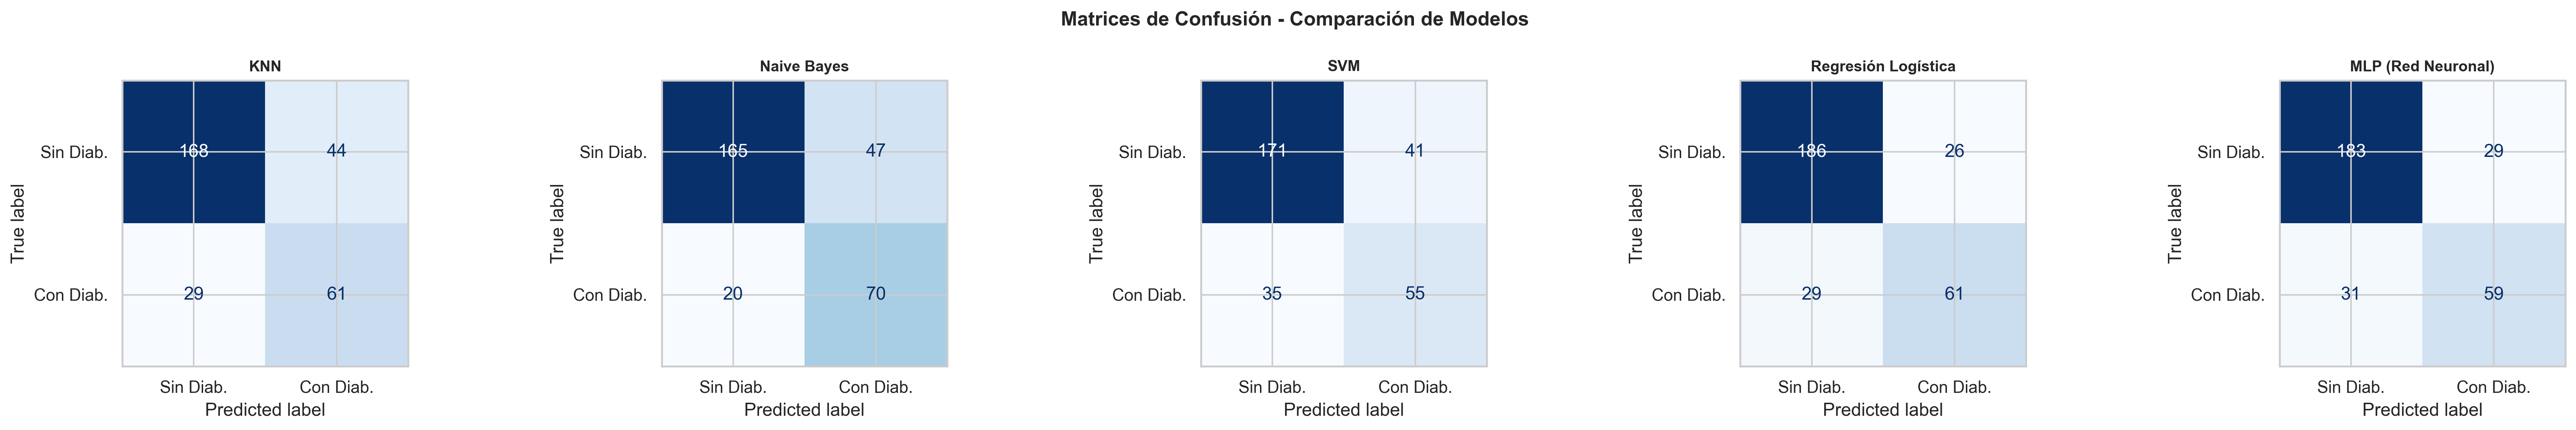
\includegraphics[width=\columnwidth]{10_matrices_confusion_modelos_base.png}
  \caption{Matrices de confusión de modelos base.}
  \label{fig:cm_base}
\end{figure}

\begin{figure}[H]
  \centering
  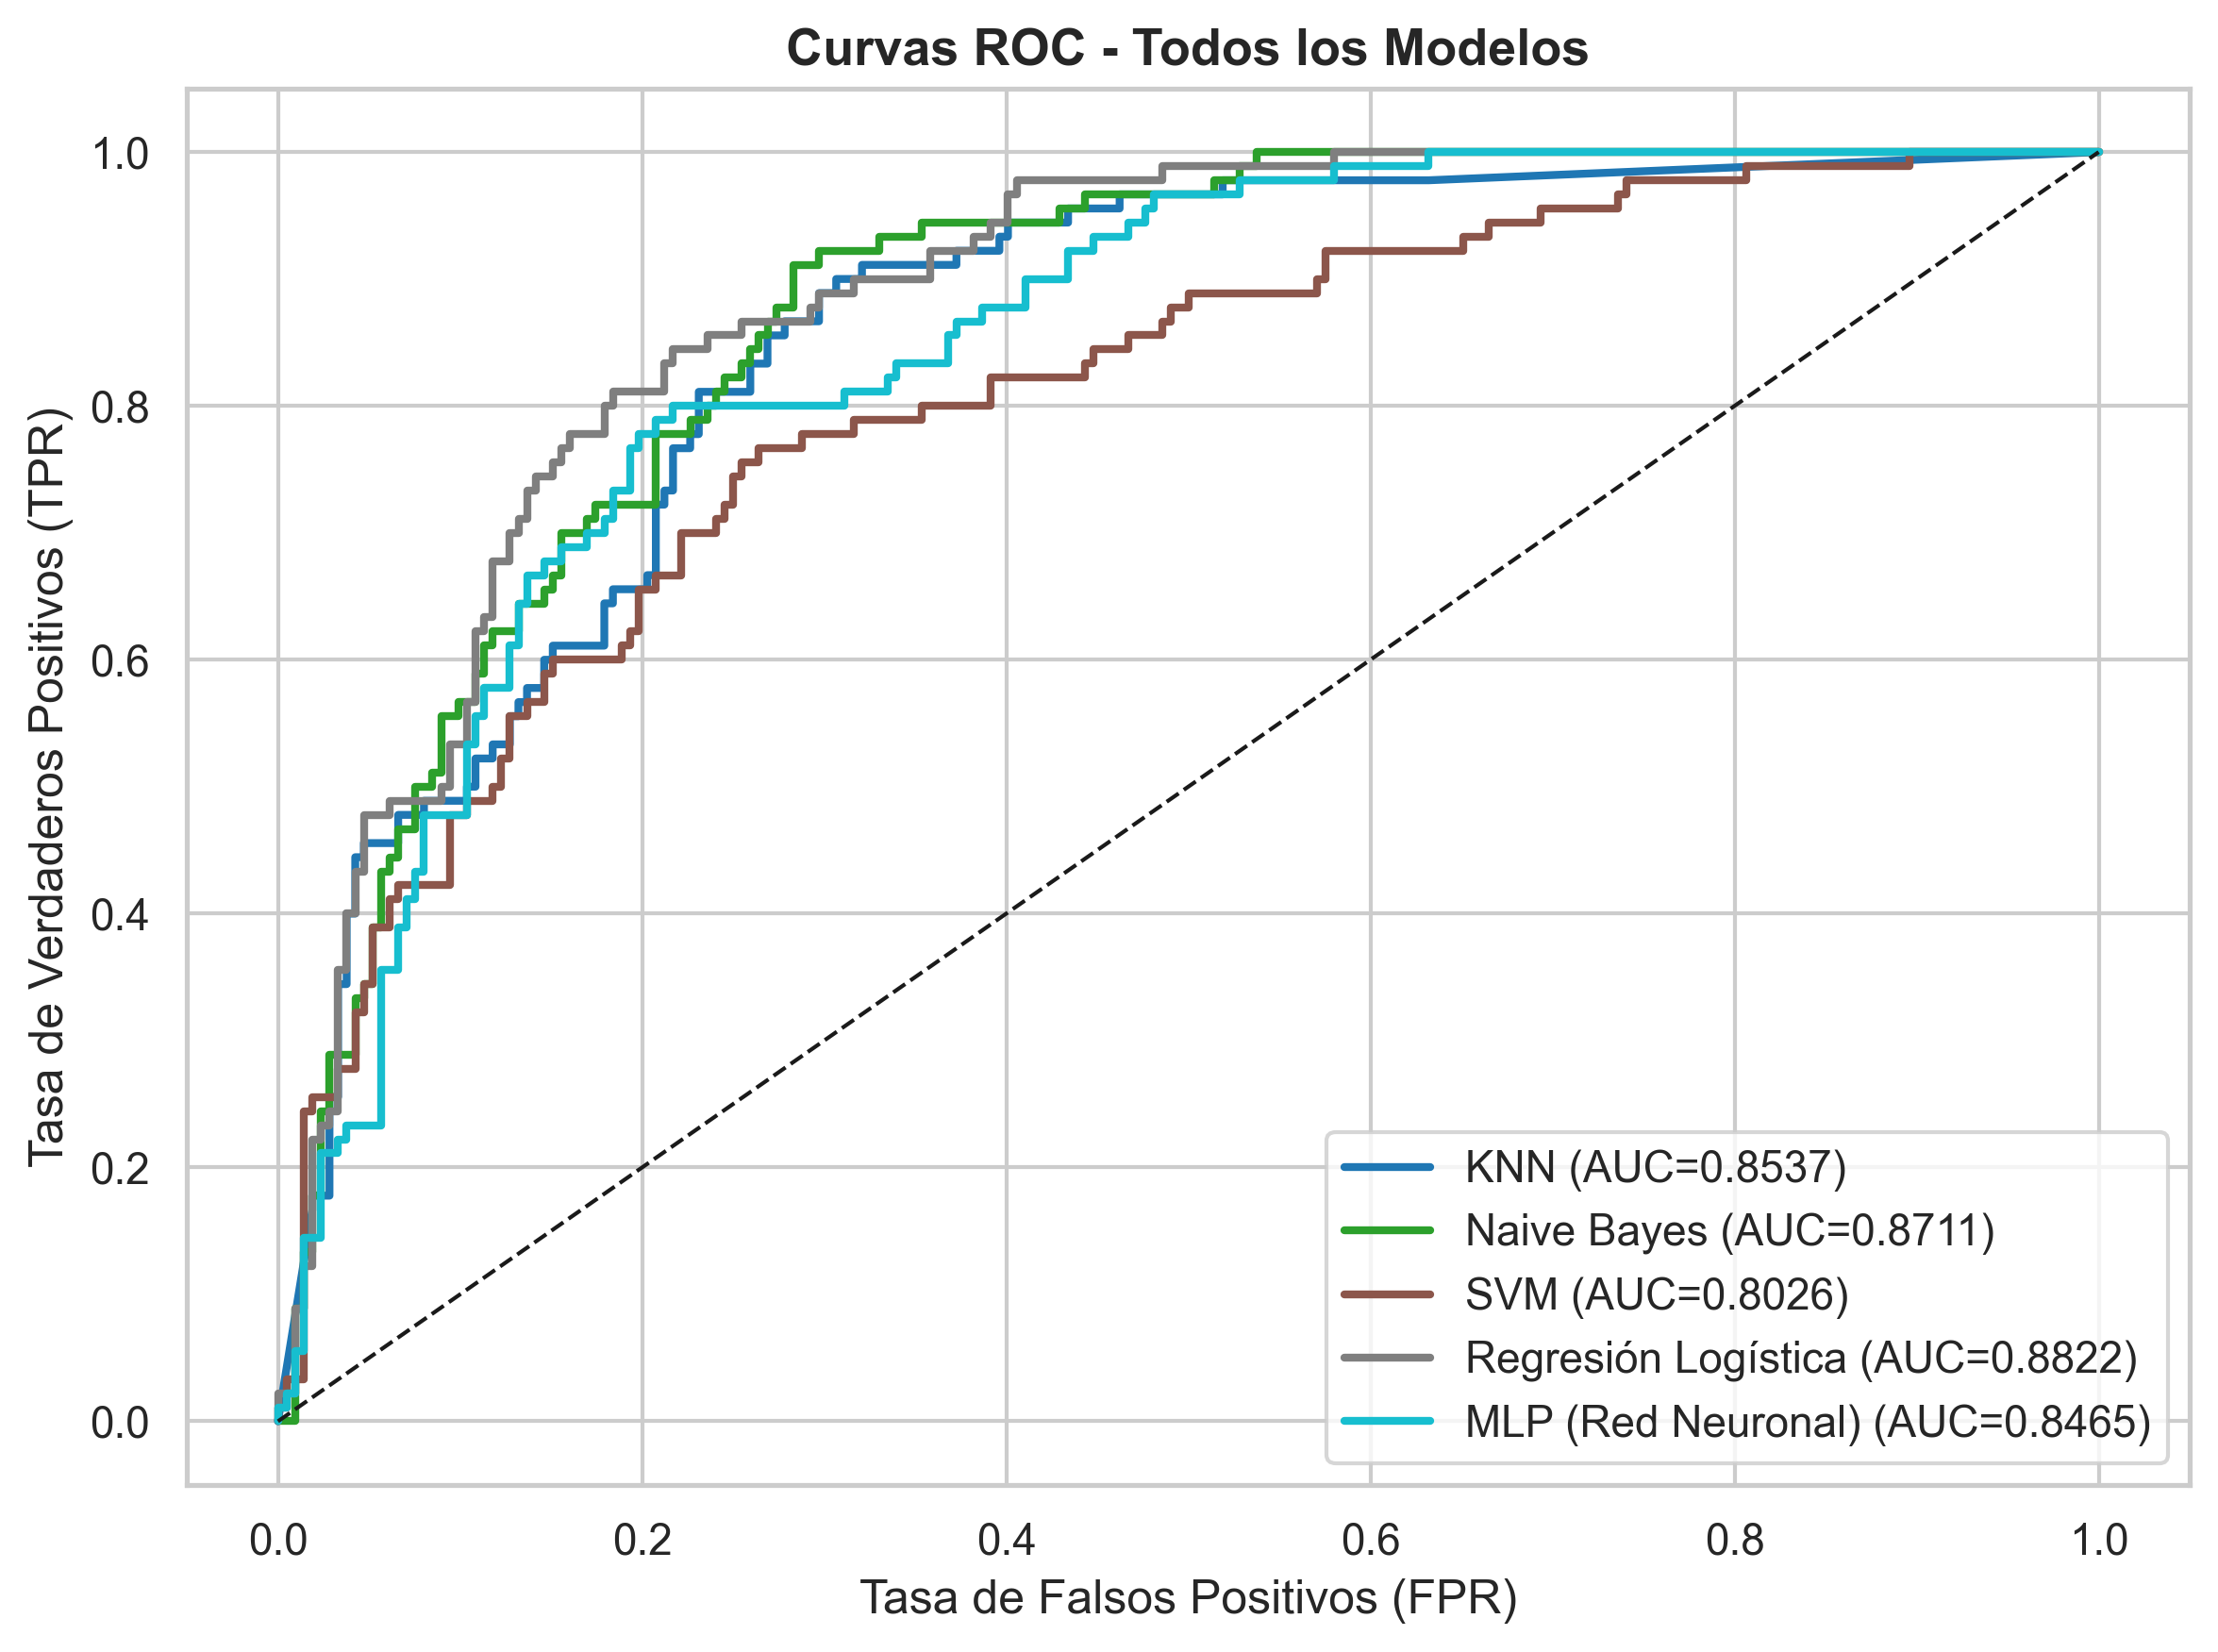
\includegraphics[width=\columnwidth]{11_roc_modelos_base.png}
  \caption{Curvas ROC de modelos base.}
  \label{fig:roc_base}
\end{figure}

\subsection{Modelos de Ensamble}

\begin{table}[H]
\centering
\caption{Métricas de modelos de ensamble en test}
\label{tab:ensambles}
\scriptsize
\setlength{\tabcolsep}{3pt}
\begin{tabular}{@{}lrrrrr@{}}
\toprule
\textbf{Modelo} & \textbf{Acc.} & \textbf{F1} & \textbf{Kappa} & \textbf{AUC} & \textbf{Gini} \\
\midrule
Bagging & \textbf{0.8344} & \textbf{0.7222} & \textbf{0.6043} & \textbf{0.8937} & \textbf{0.7873} \\
AdaBoost & 0.8013 & 0.6667 & 0.5252 & 0.8499 & 0.6999 \\
Gradient Boosting & 0.8013 & 0.6629 & 0.5221 & 0.8596 & 0.7193 \\
XGBoost & 0.8146 & 0.6989 & 0.5652 & 0.8738 & 0.7476 \\
LightGBM & 0.8278 & 0.7204 & 0.5962 & 0.8651 & 0.7302 \\
\bottomrule
\end{tabular}
\end{table}

La respuesta a esa pregunta aparece en la Tabla~\ref{tab:ensambles}: al pasar a los ensambles, Bagging de árboles tomó la delantera y se convirtió, además, en el mejor modelo de todo el estudio, encabezando las cinco métricas reportadas (accuracy, F1, kappa, ROC AUC y Gini). La competencia, sin embargo, fue estrecha ---LightGBM quedó muy cerca en F1 y accuracy, y XGBoost fue el segundo mejor en ROC AUC---, lo que ya anticipa que la ventaja del ganador no es amplia y conviene contrastarla con un enfoque aún más elaborado.

\begin{figure}[H]
  \centering
  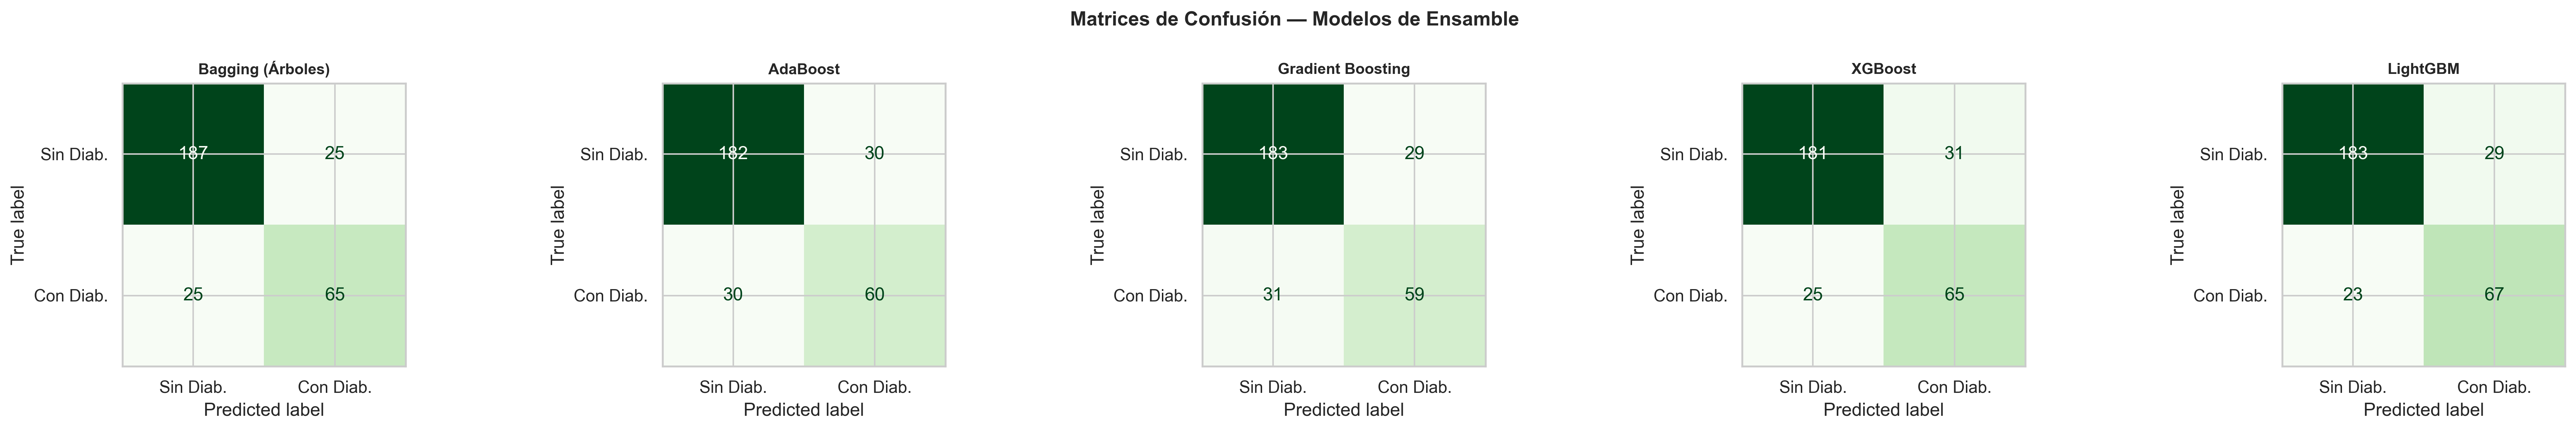
\includegraphics[width=\columnwidth]{16_matrices_confusion_ensambles.png}
  \caption{Matrices de confusión de modelos de ensamble.}
  \label{fig:cm_ensambles}
\end{figure}

\begin{figure}[H]
  \centering
  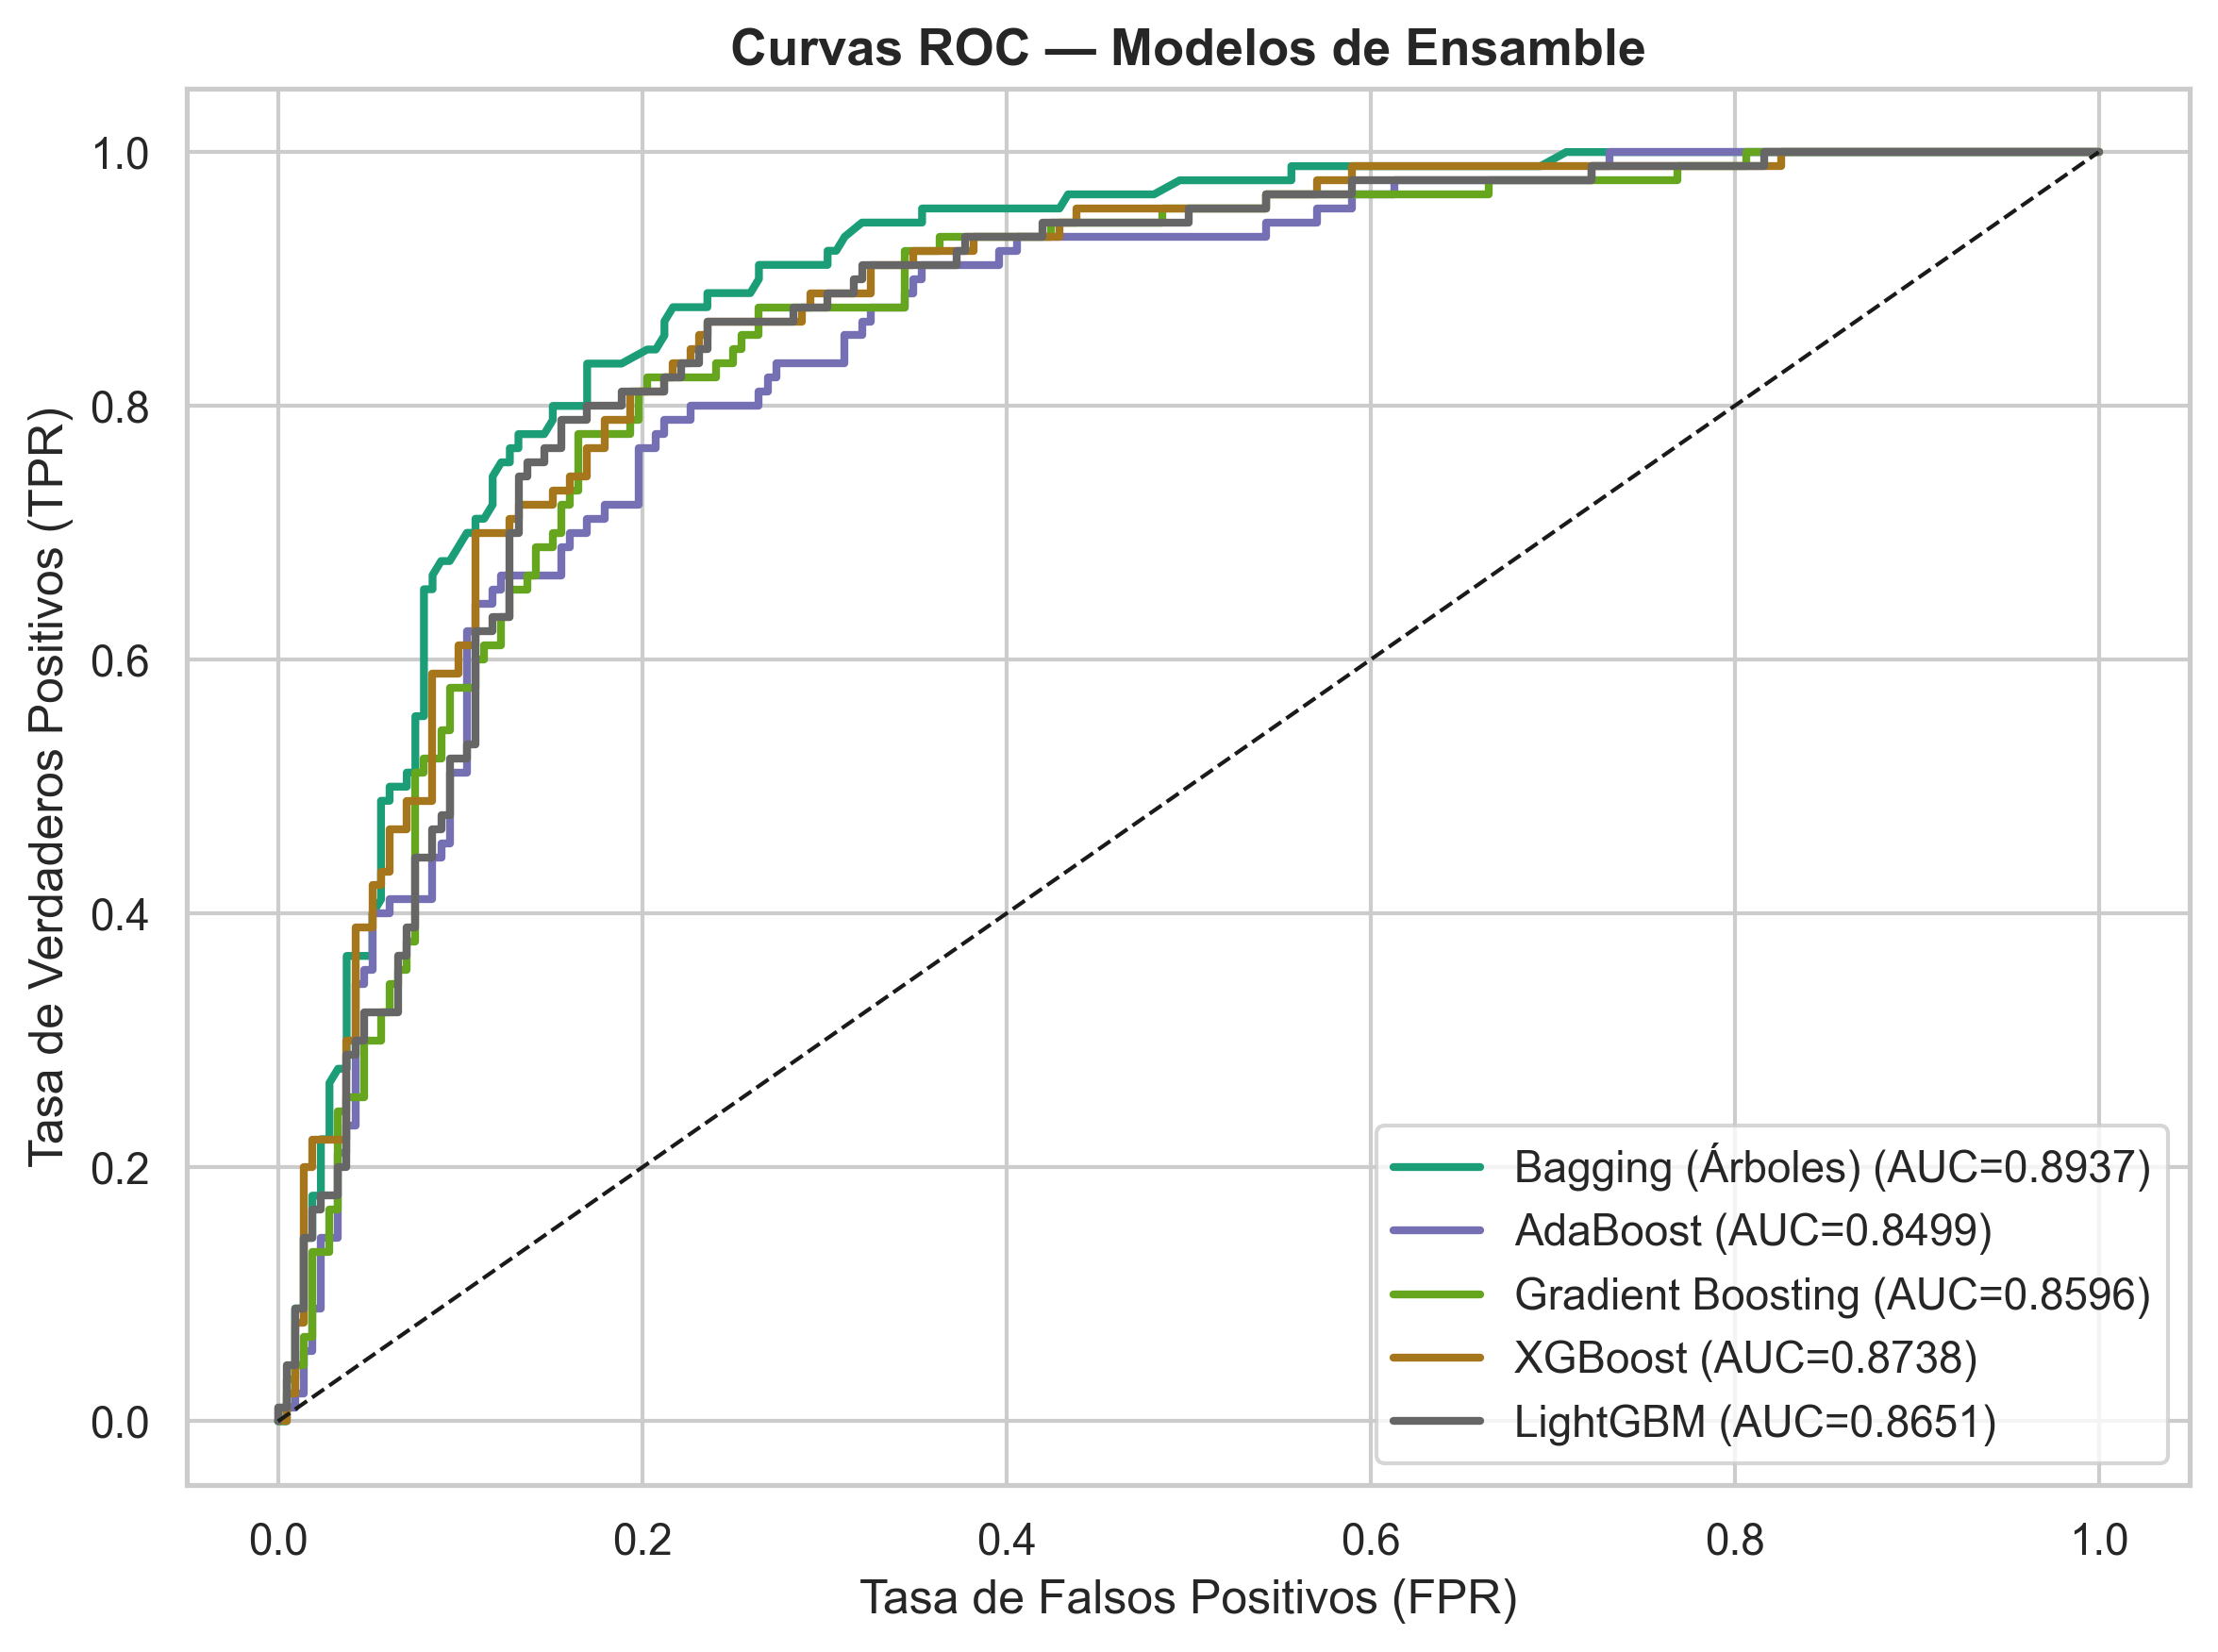
\includegraphics[width=\columnwidth]{17_roc_ensambles.png}
  \caption{Curvas ROC de modelos de ensamble.}
  \label{fig:roc_ensambles}
\end{figure}

\subsection{Comparación Global y Stacking}

\begin{table}[H]
\centering
\caption{Ranking final por ROC AUC}
\label{tab:ranking}
\scriptsize
\begin{tabular}{@{}rlrr@{}}
\toprule
\textbf{Rank} & \textbf{Modelo} & \textbf{AUC} & \textbf{F1} \\
\midrule
1 & Bagging de árboles & \textbf{0.8937} & \textbf{0.7222} \\
2 & Stacking Top-3 & 0.8889 & 0.7174 \\
3 & Regresión Logística & 0.8822 & 0.6893 \\
4 & XGBoost & 0.8738 & 0.6989 \\
5 & Naive Bayes & 0.8711 & 0.6763 \\
6 & LightGBM & 0.8651 & 0.7204 \\
7 & Gradient Boosting & 0.8596 & 0.6629 \\
8 & KNN & 0.8537 & 0.6256 \\
9 & AdaBoost & 0.8499 & 0.6667 \\
10 & MLP & 0.8465 & 0.6629 \\
11 & SVM & 0.8026 & 0.5914 \\
\bottomrule
\end{tabular}
\end{table}

\begin{figure}[H]
  \centering
  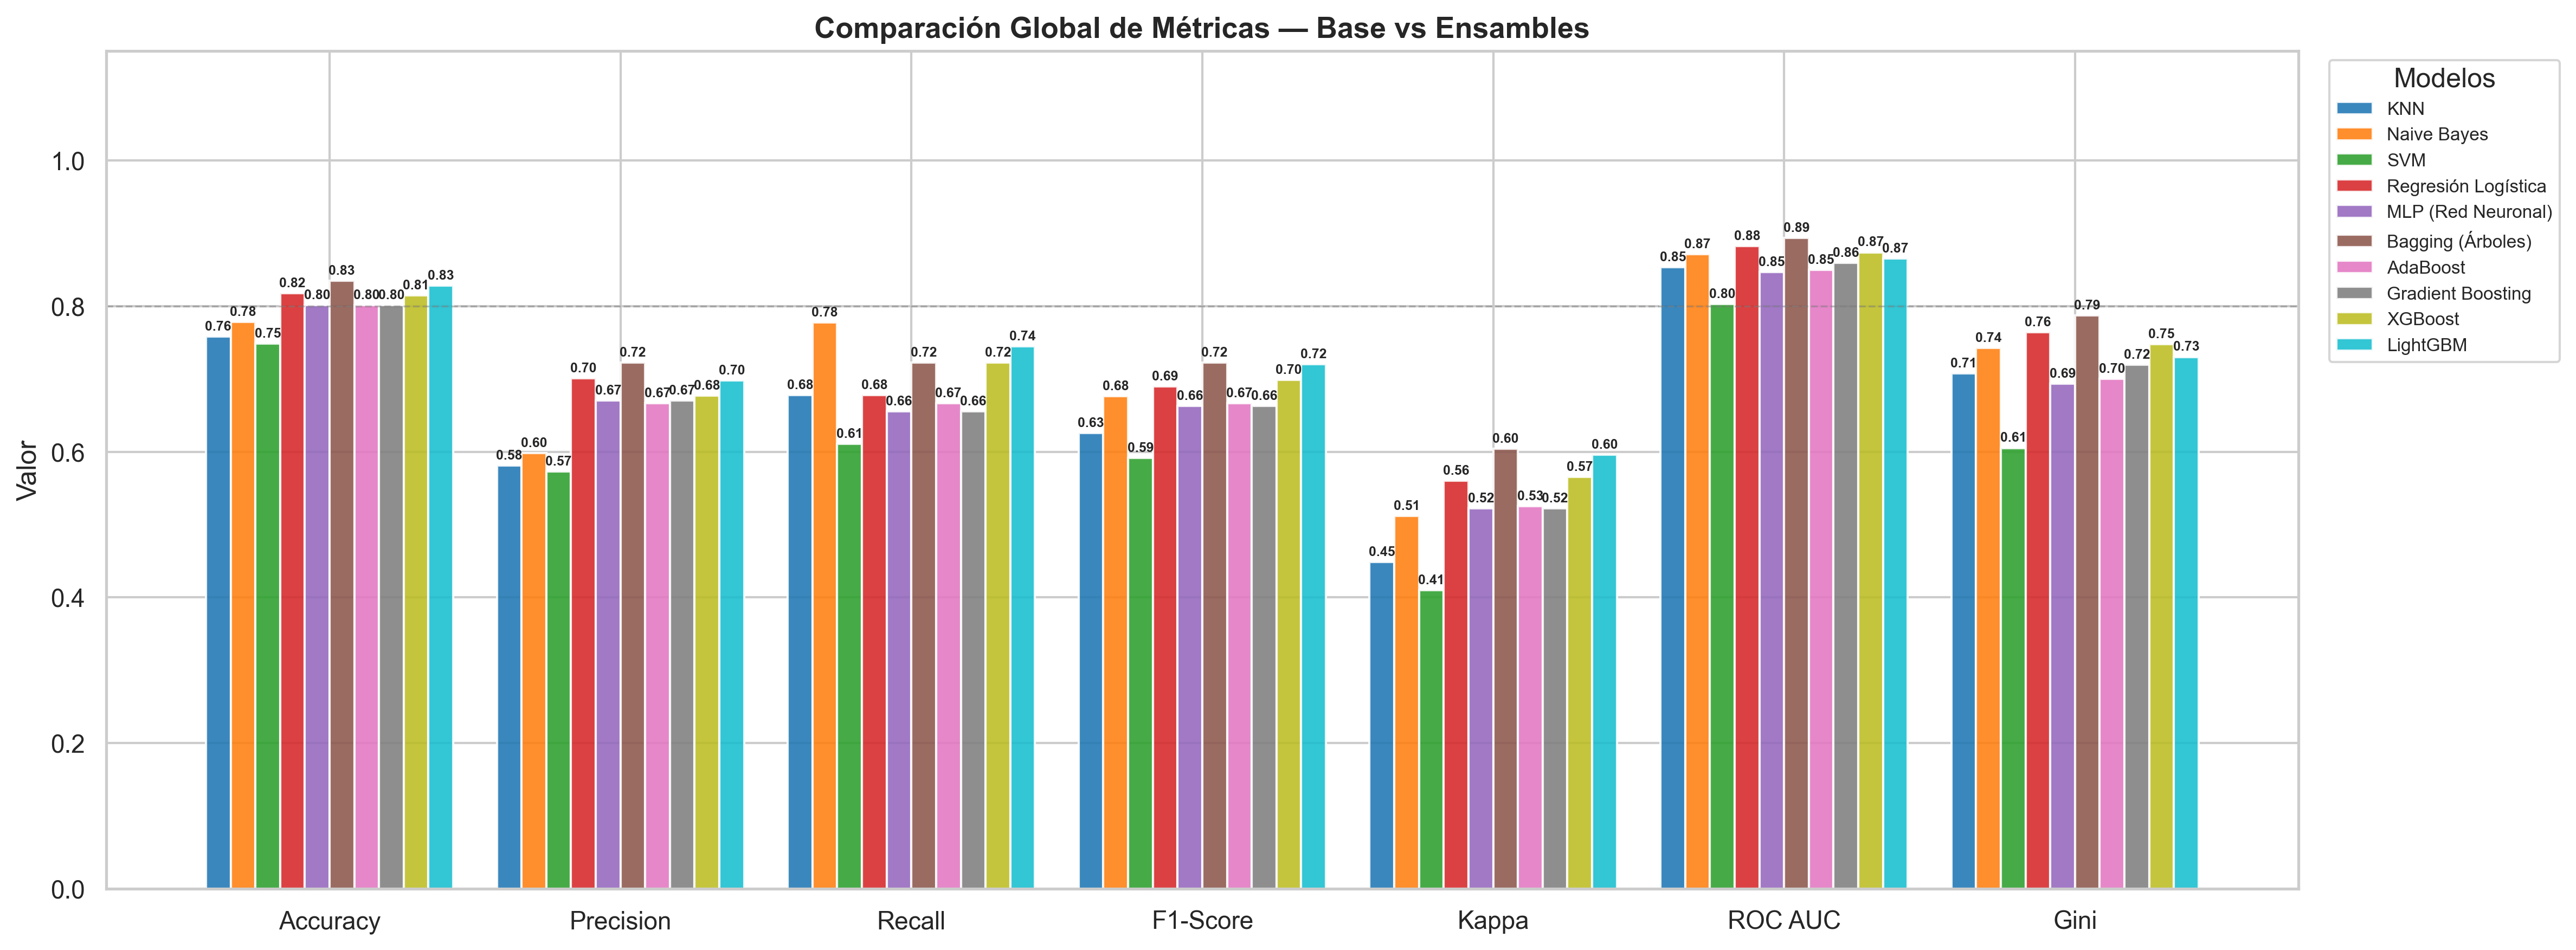
\includegraphics[width=\columnwidth]{20_metricas_globales_modelos.png}
  \caption{Comparación global de métricas entre modelos.}
  \label{fig:métricas_globales}
\end{figure}

Ese enfoque más elaborado es el Stacking Top-3, que combinó los tres modelos con mejor ROC AUC en validación cruzada (LightGBM, Bagging y XGBoost) sobre una Regresión Logística como meta-aprendiz. El resultado, no obstante, refuerza lo anterior: alcanzó un ROC AUC de 0.8889, apenas 0.0048 por debajo del Bagging individual. El ranking global (Tabla~\ref{tab:ranking}) lo confirma dejando al Bagging en primer lugar. La lectura es clara: añadir complejidad no rindió mejora, de modo que se conserva el Bagging como modelo final por ser igual de preciso y más simple de operar.

\begin{figure}[H]
  \centering
  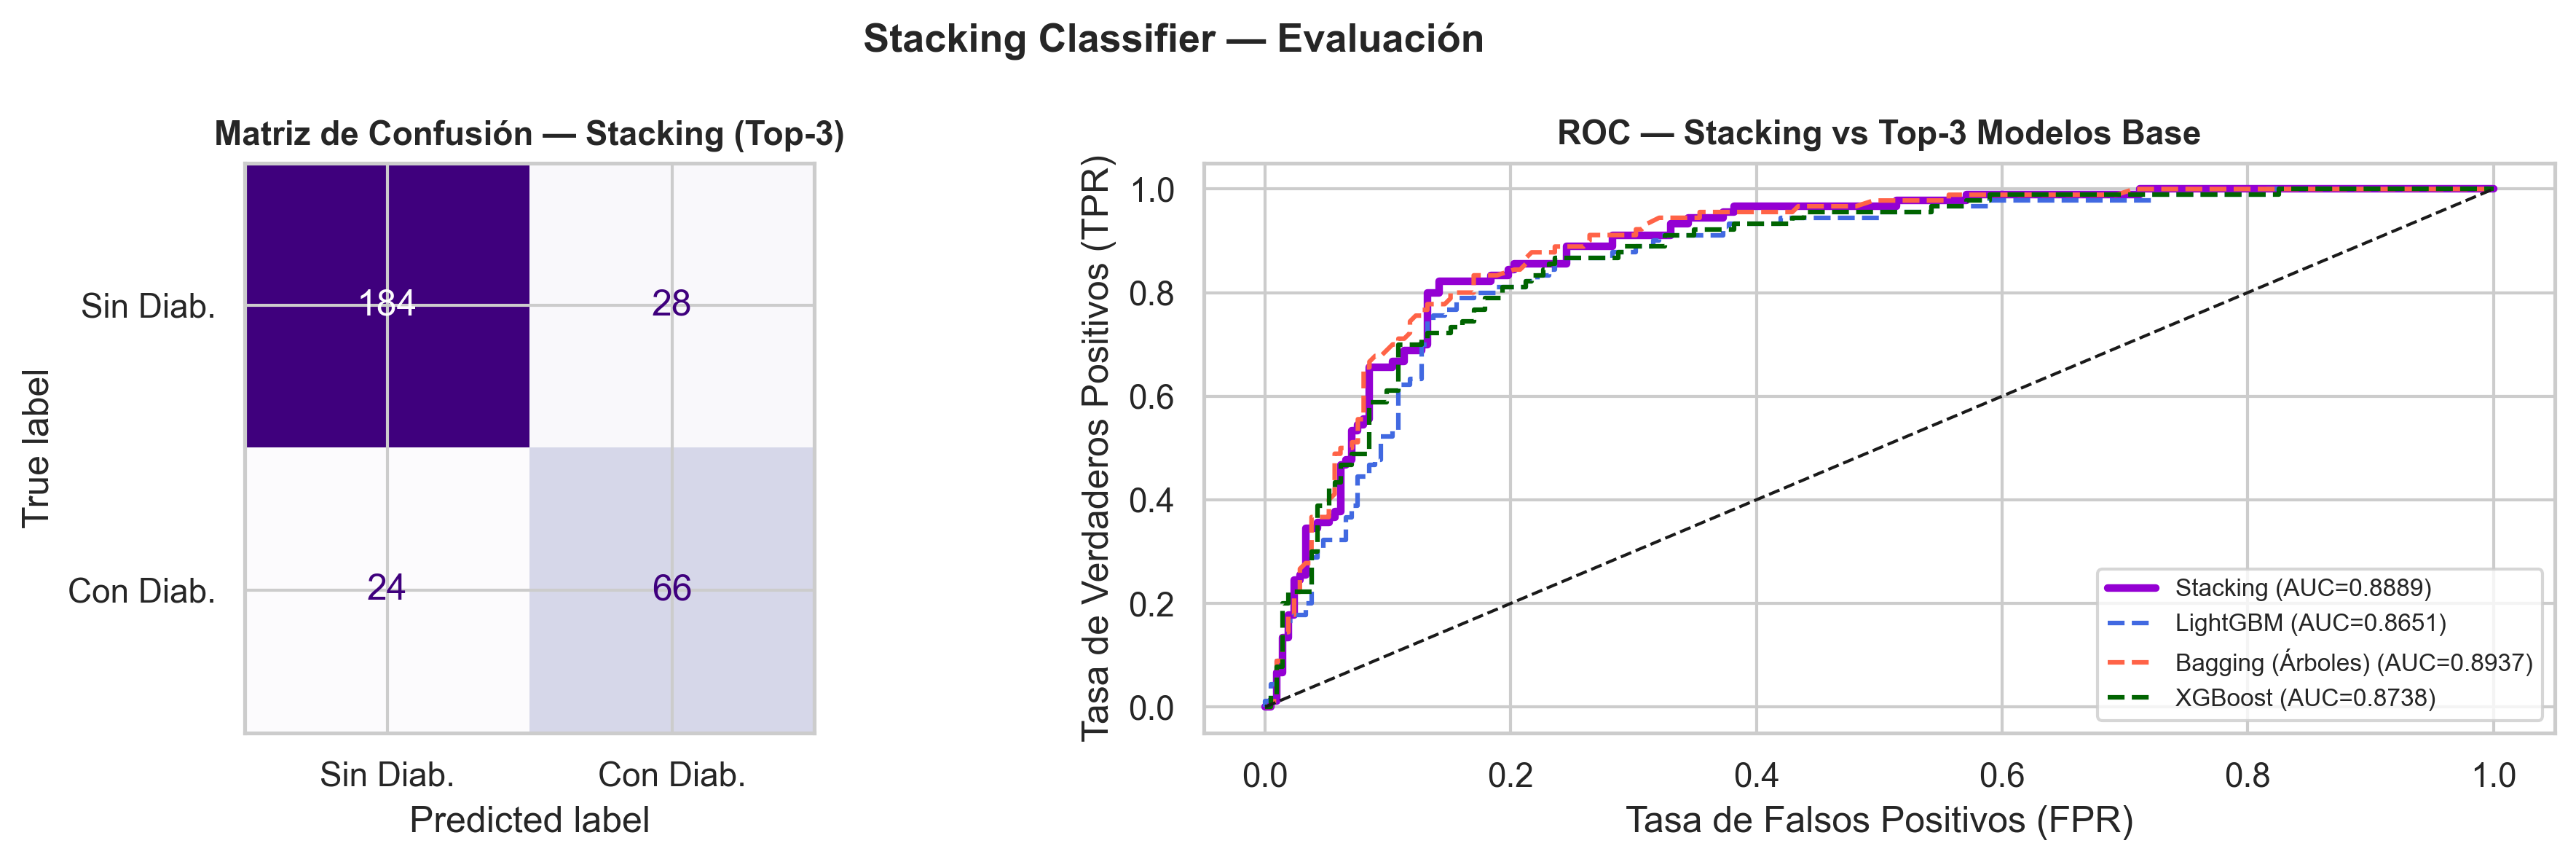
\includegraphics[width=\columnwidth]{21_stacking_matriz_roc.png}
  \caption{Evaluación del Stacking Top-3: matriz de confusión y curva ROC.}
  \label{fig:stacking}
\end{figure}

\subsection{Lift por Decil}

El análisis de lift evalúa la utilidad práctica del score predictivo para priorizar pacientes de mayor riesgo. Un lift superior a 1 indica que el modelo captura más casos positivos que una selección aleatoria. Las curvas de lift muestran que los modelos con mejor ranking concentran una mayor tasa de positivos en los primeros deciles. Para el modelo ganador (Bagging), el decil de mayor score (10\% superior) alcanza una tasa de positivos de 77.4\% frente a una tasa base de 29.8\% ---un lift de 2.60--- y captura el 26.7\% de todos los casos con diabetes del test; al ampliar al 20\% de mayor score se captura el 51.1\% de los positivos. Estas cifras cuantifican la utilidad del score para priorización.

\begin{figure}[H]
  \centering
  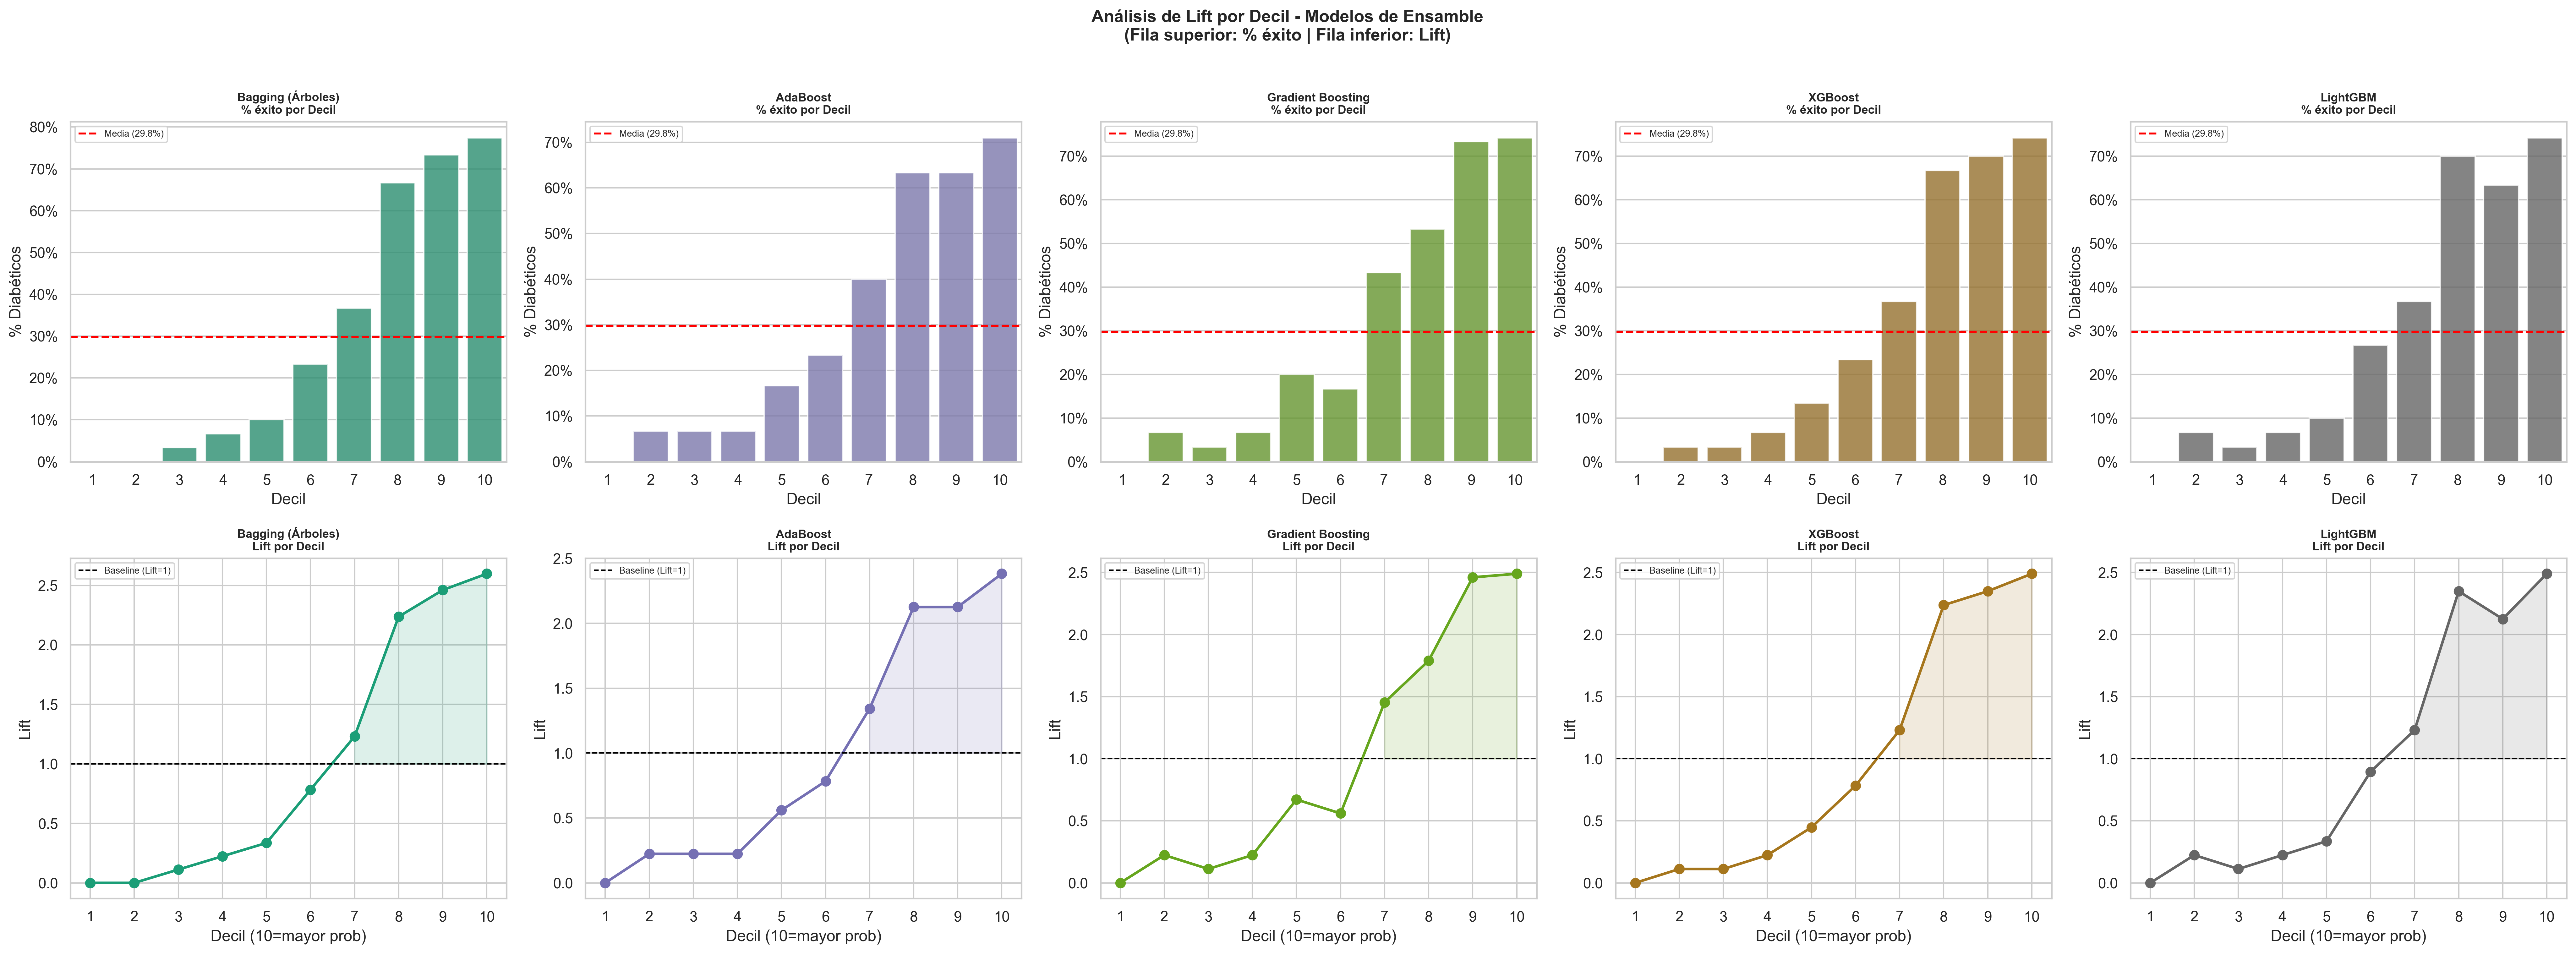
\includegraphics[width=\columnwidth]{18_lift_deciles_ensambles.png}
  \caption{Lift por decil en modelos de ensamble.}
  \label{fig:lift_deciles}
\end{figure}

\begin{figure}[H]
  \centering
  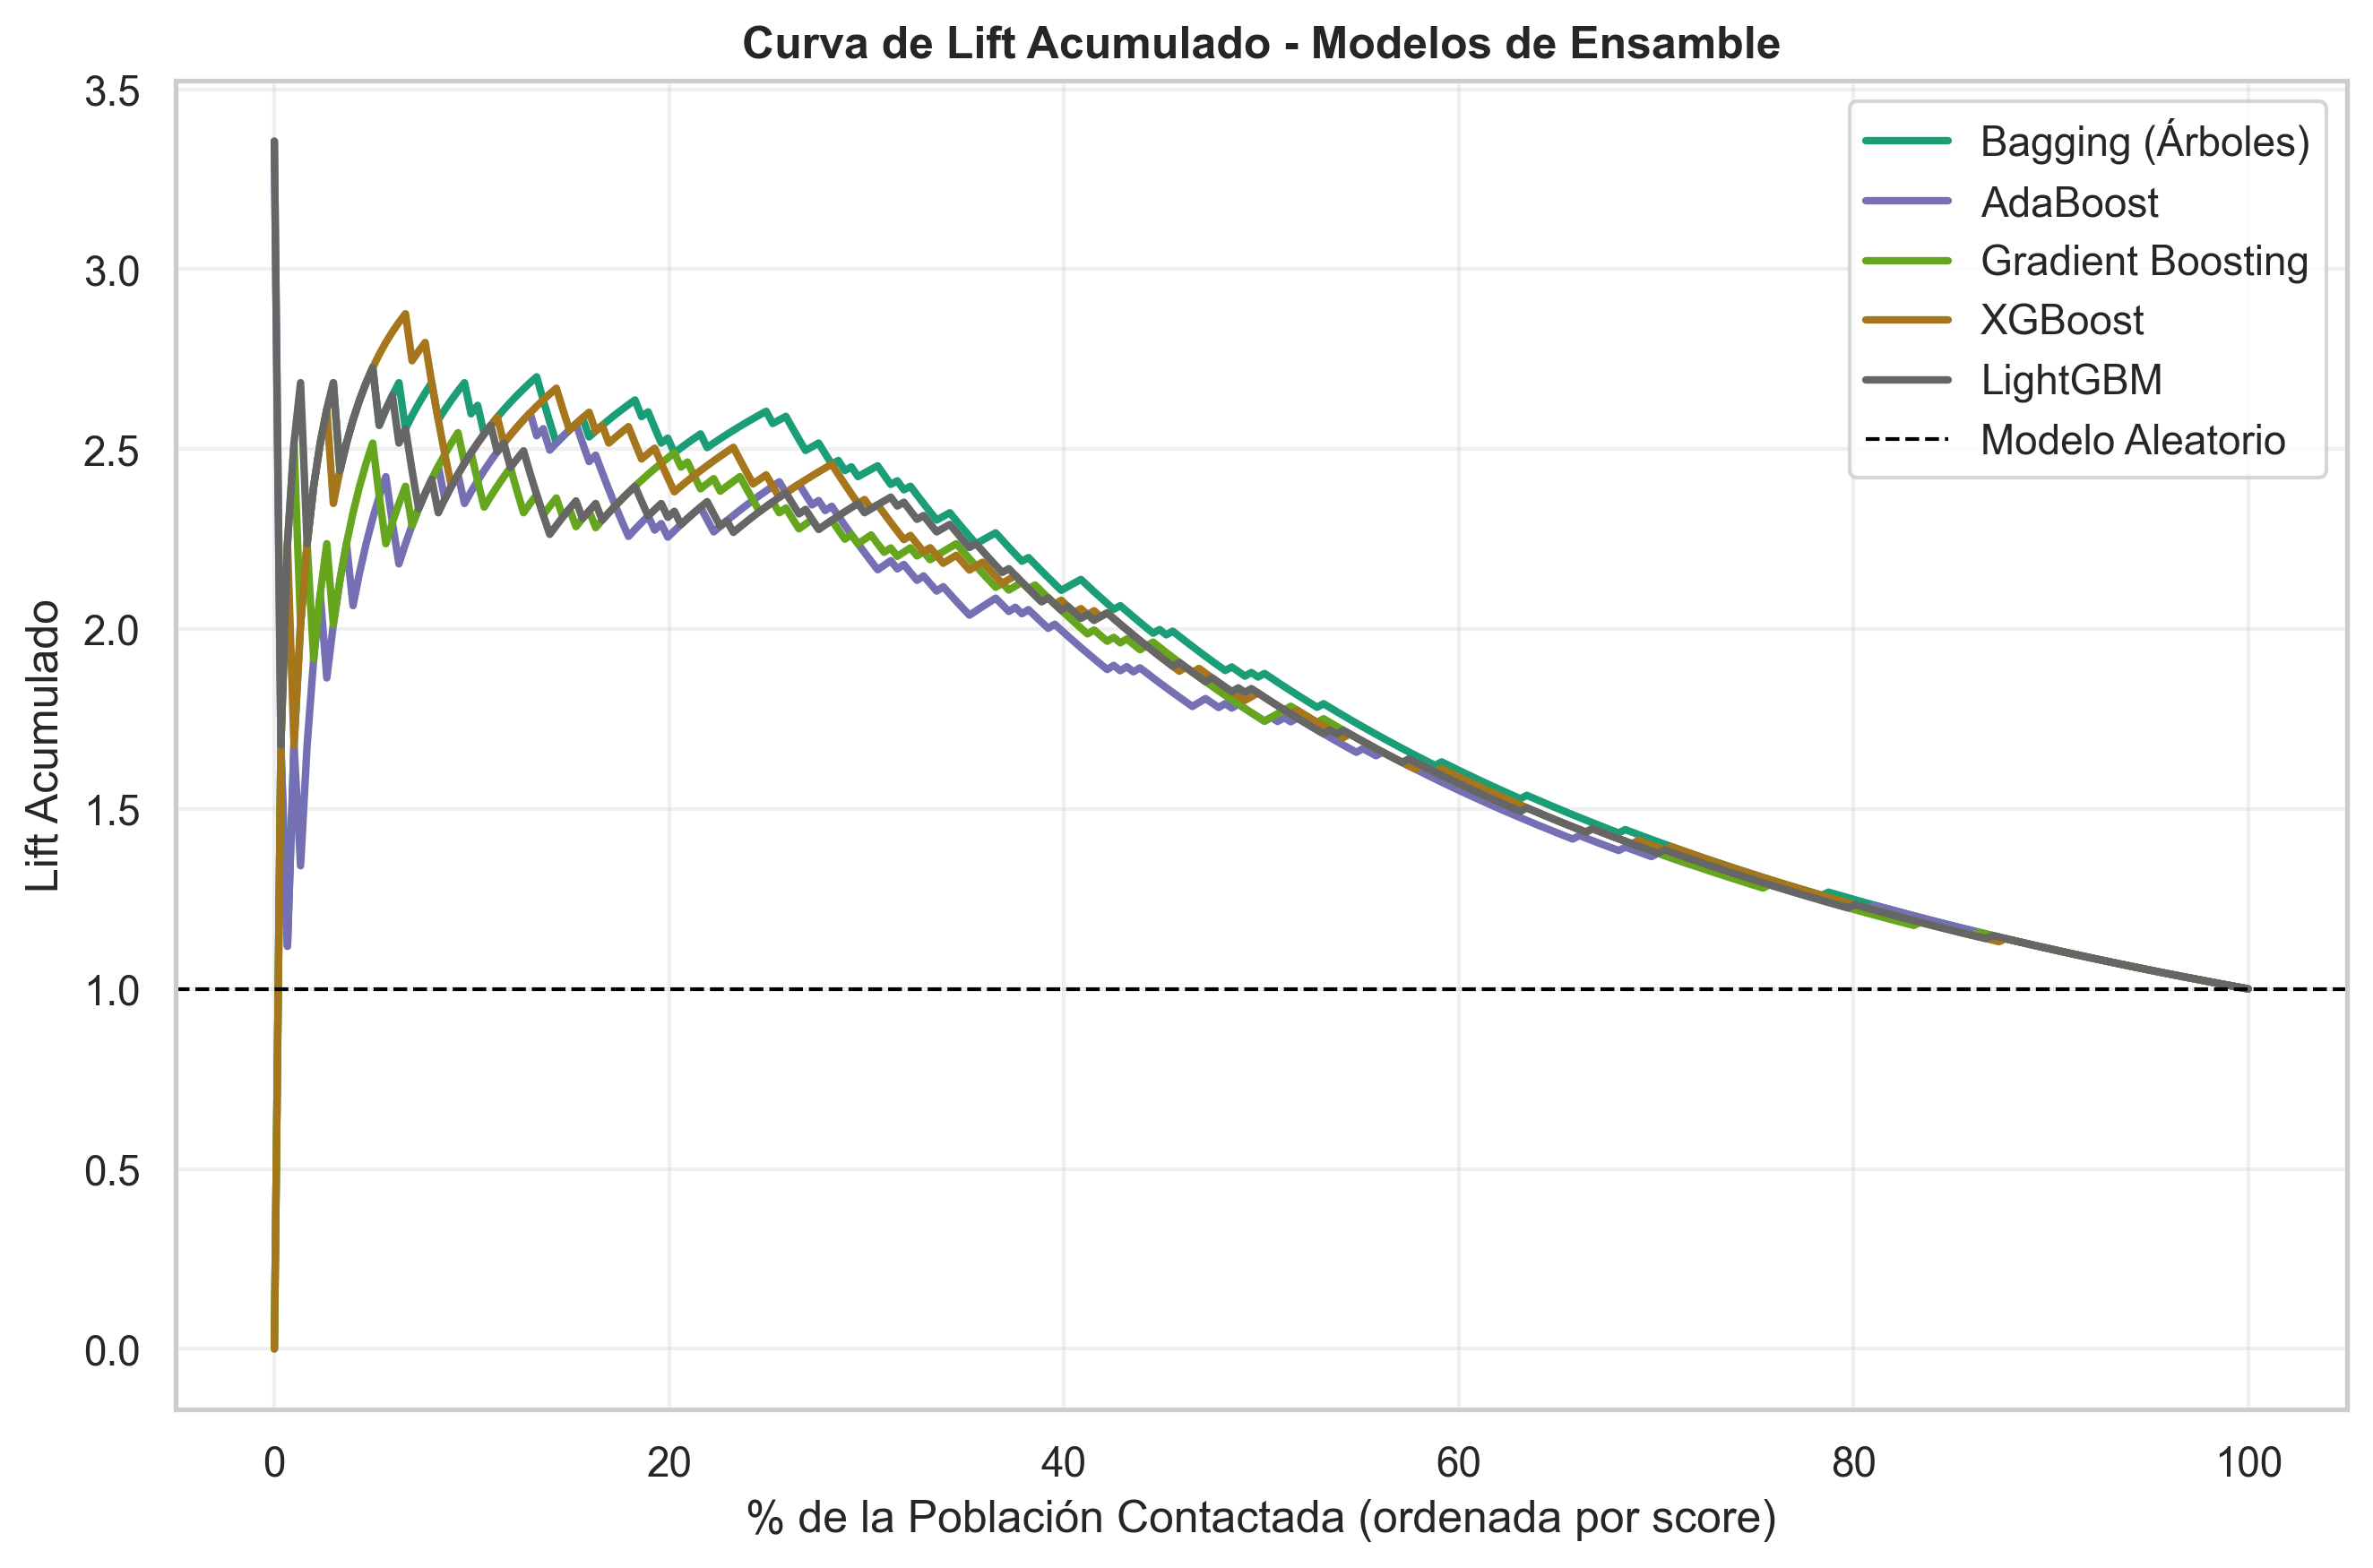
\includegraphics[width=\columnwidth]{19_lift_acumulado_ensambles.png}
  \caption{Lift acumulado en modelos de ensamble.}
  \label{fig:lift_acumulado}
\end{figure}

Desde una perspectiva operativa, este tipo de análisis es especialmente útil en salud pública: si los recursos diagnósticos son limitados, un modelo con buen lift permite priorizar a quienes tienen mayor probabilidad de diabetes para confirmación clínica.

\section{Interpretabilidad}

La interpretabilidad responde a una pregunta que la métrica de desempeño no contesta: \emph{por qué} el modelo predice lo que predice. Se trabajó con SHAP, un enfoque basado en valores de Shapley que descompone cada predicción en la contribución individual de cada variable \cite{lundberg2017}. Dado que el modelo ganador Bagging de árboles de \code{scikit-learn} no es compatible directamente con \code{TreeExplainer}, se usó \code{KernelExplainer} para explicar la probabilidad de la clase positiva del ganador, con 80 observaciones de entrenamiento como background y 40 instancias de test explicadas (\code{nsamples}$=200$); esta configuración acotada responde al alto costo del método basado en muestreo. Además, se incluyó un análisis complementario con \code{TreeExplainer} sobre XGBoost, por ser el mejor modelo de árbol compatible con ese método, lo que permite verificar si las conclusiones se sostienen entre modelos distintos.

\begin{figure}[H]
  \centering
  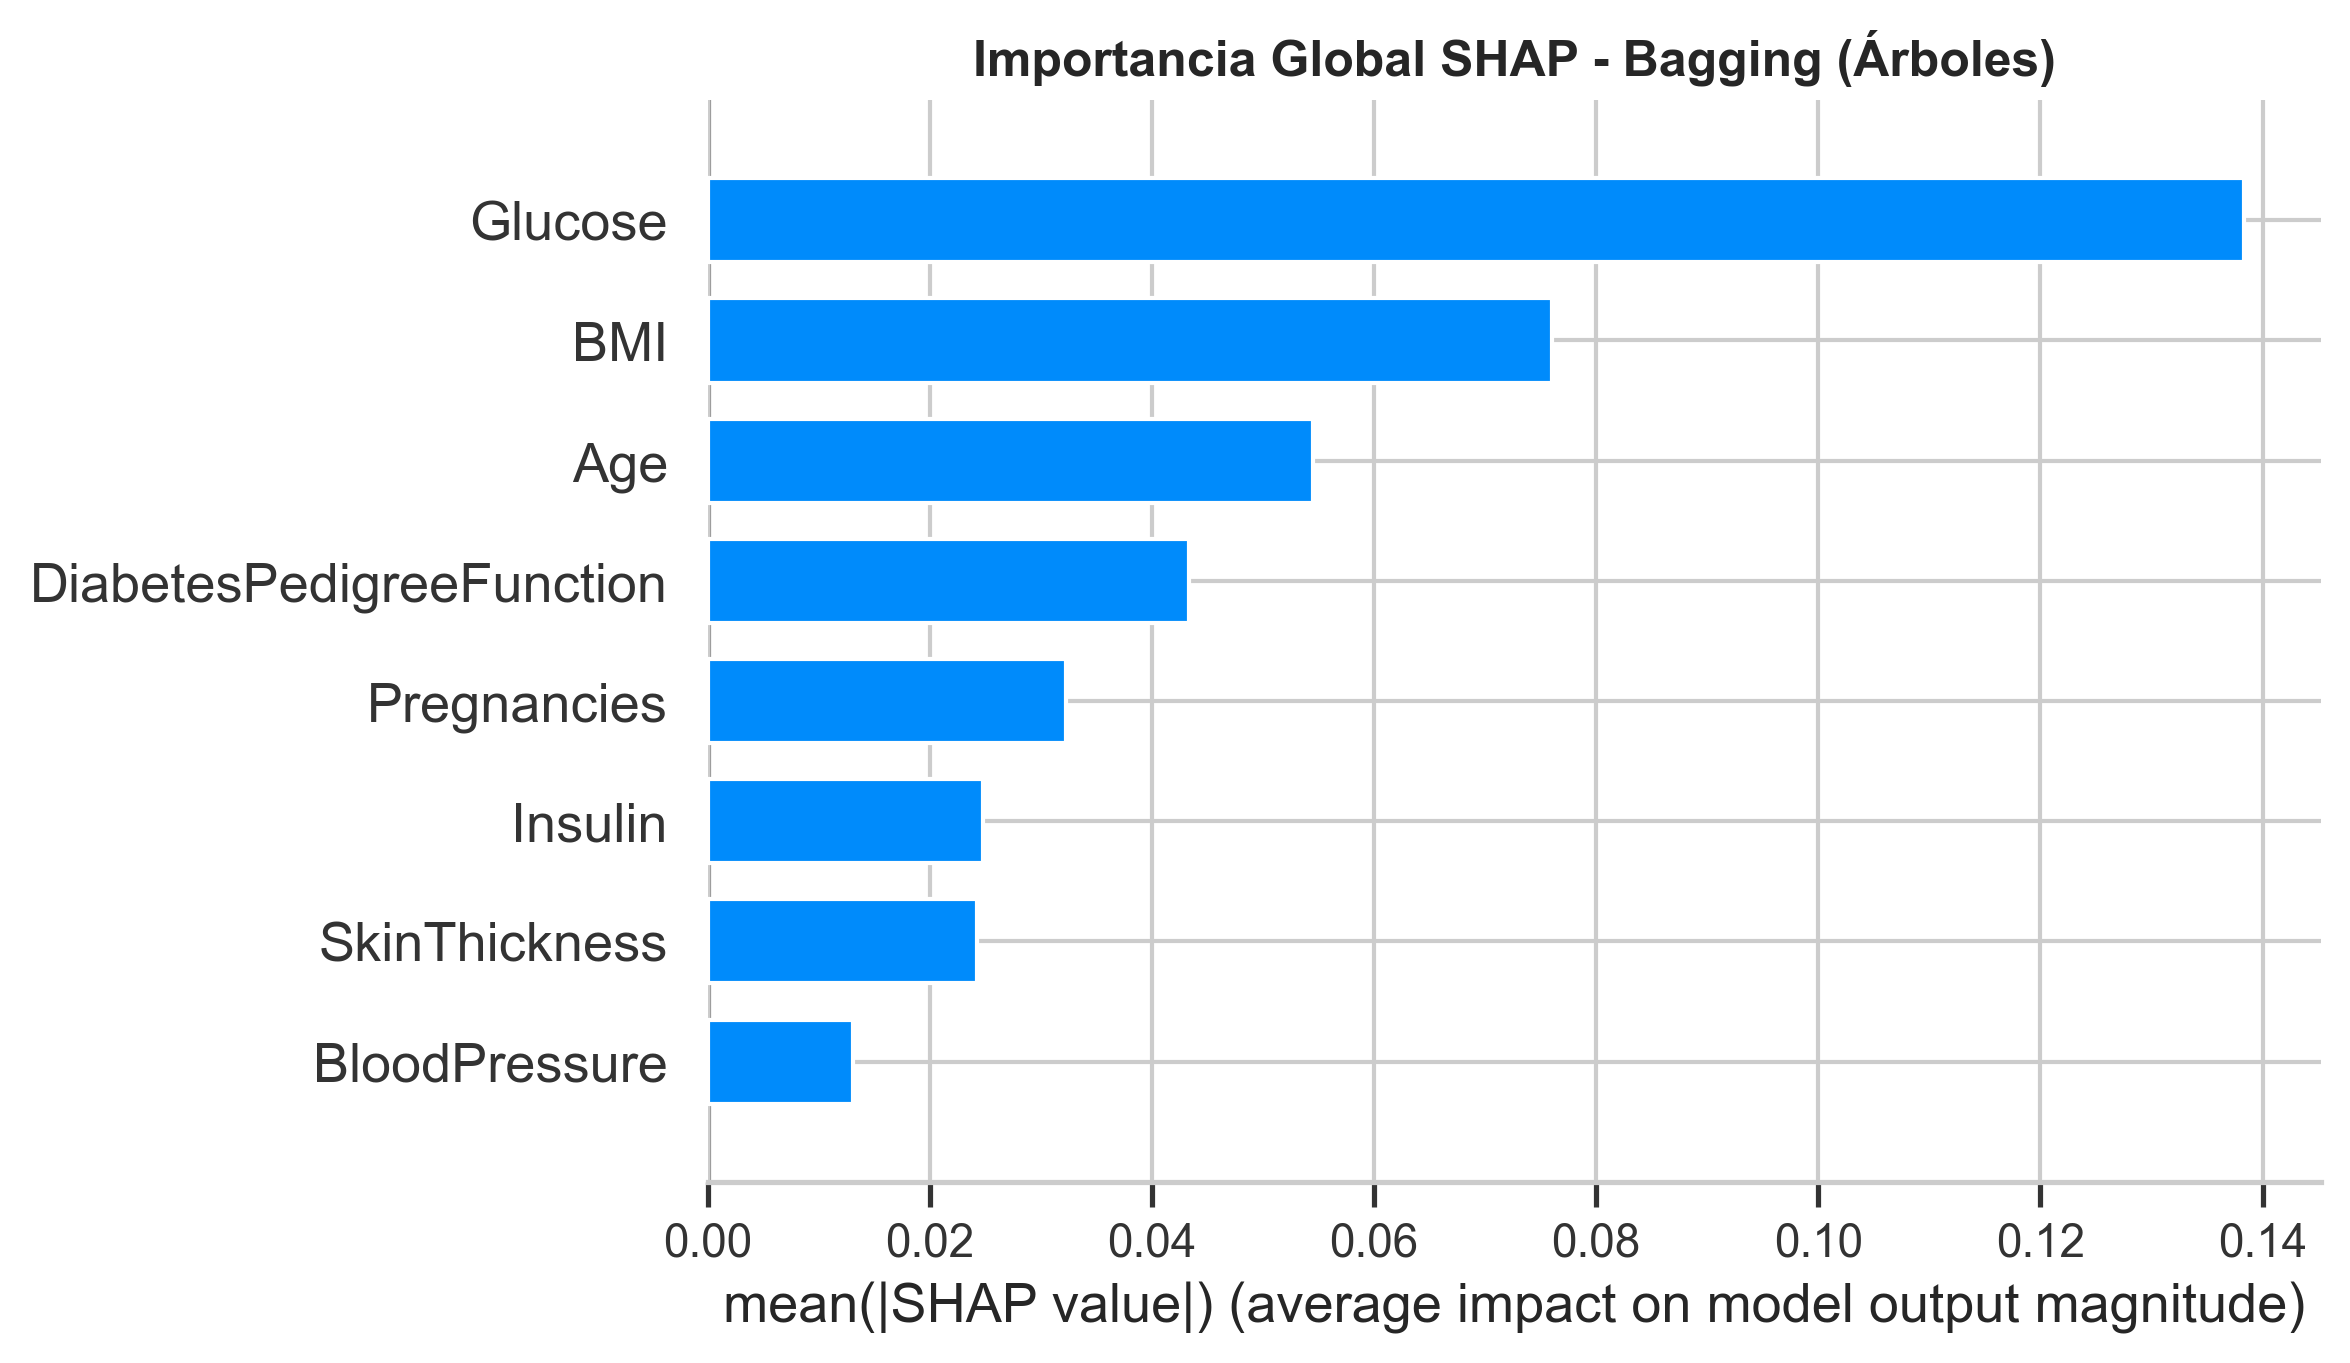
\includegraphics[width=\columnwidth]{22_ganador_importancia_global_shap.png}
  \caption{Importancia global SHAP del modelo ganador: Bagging de árboles.}
  \label{fig:shap_bar_bagging}
\end{figure}

\begin{figure}[H]
  \centering
  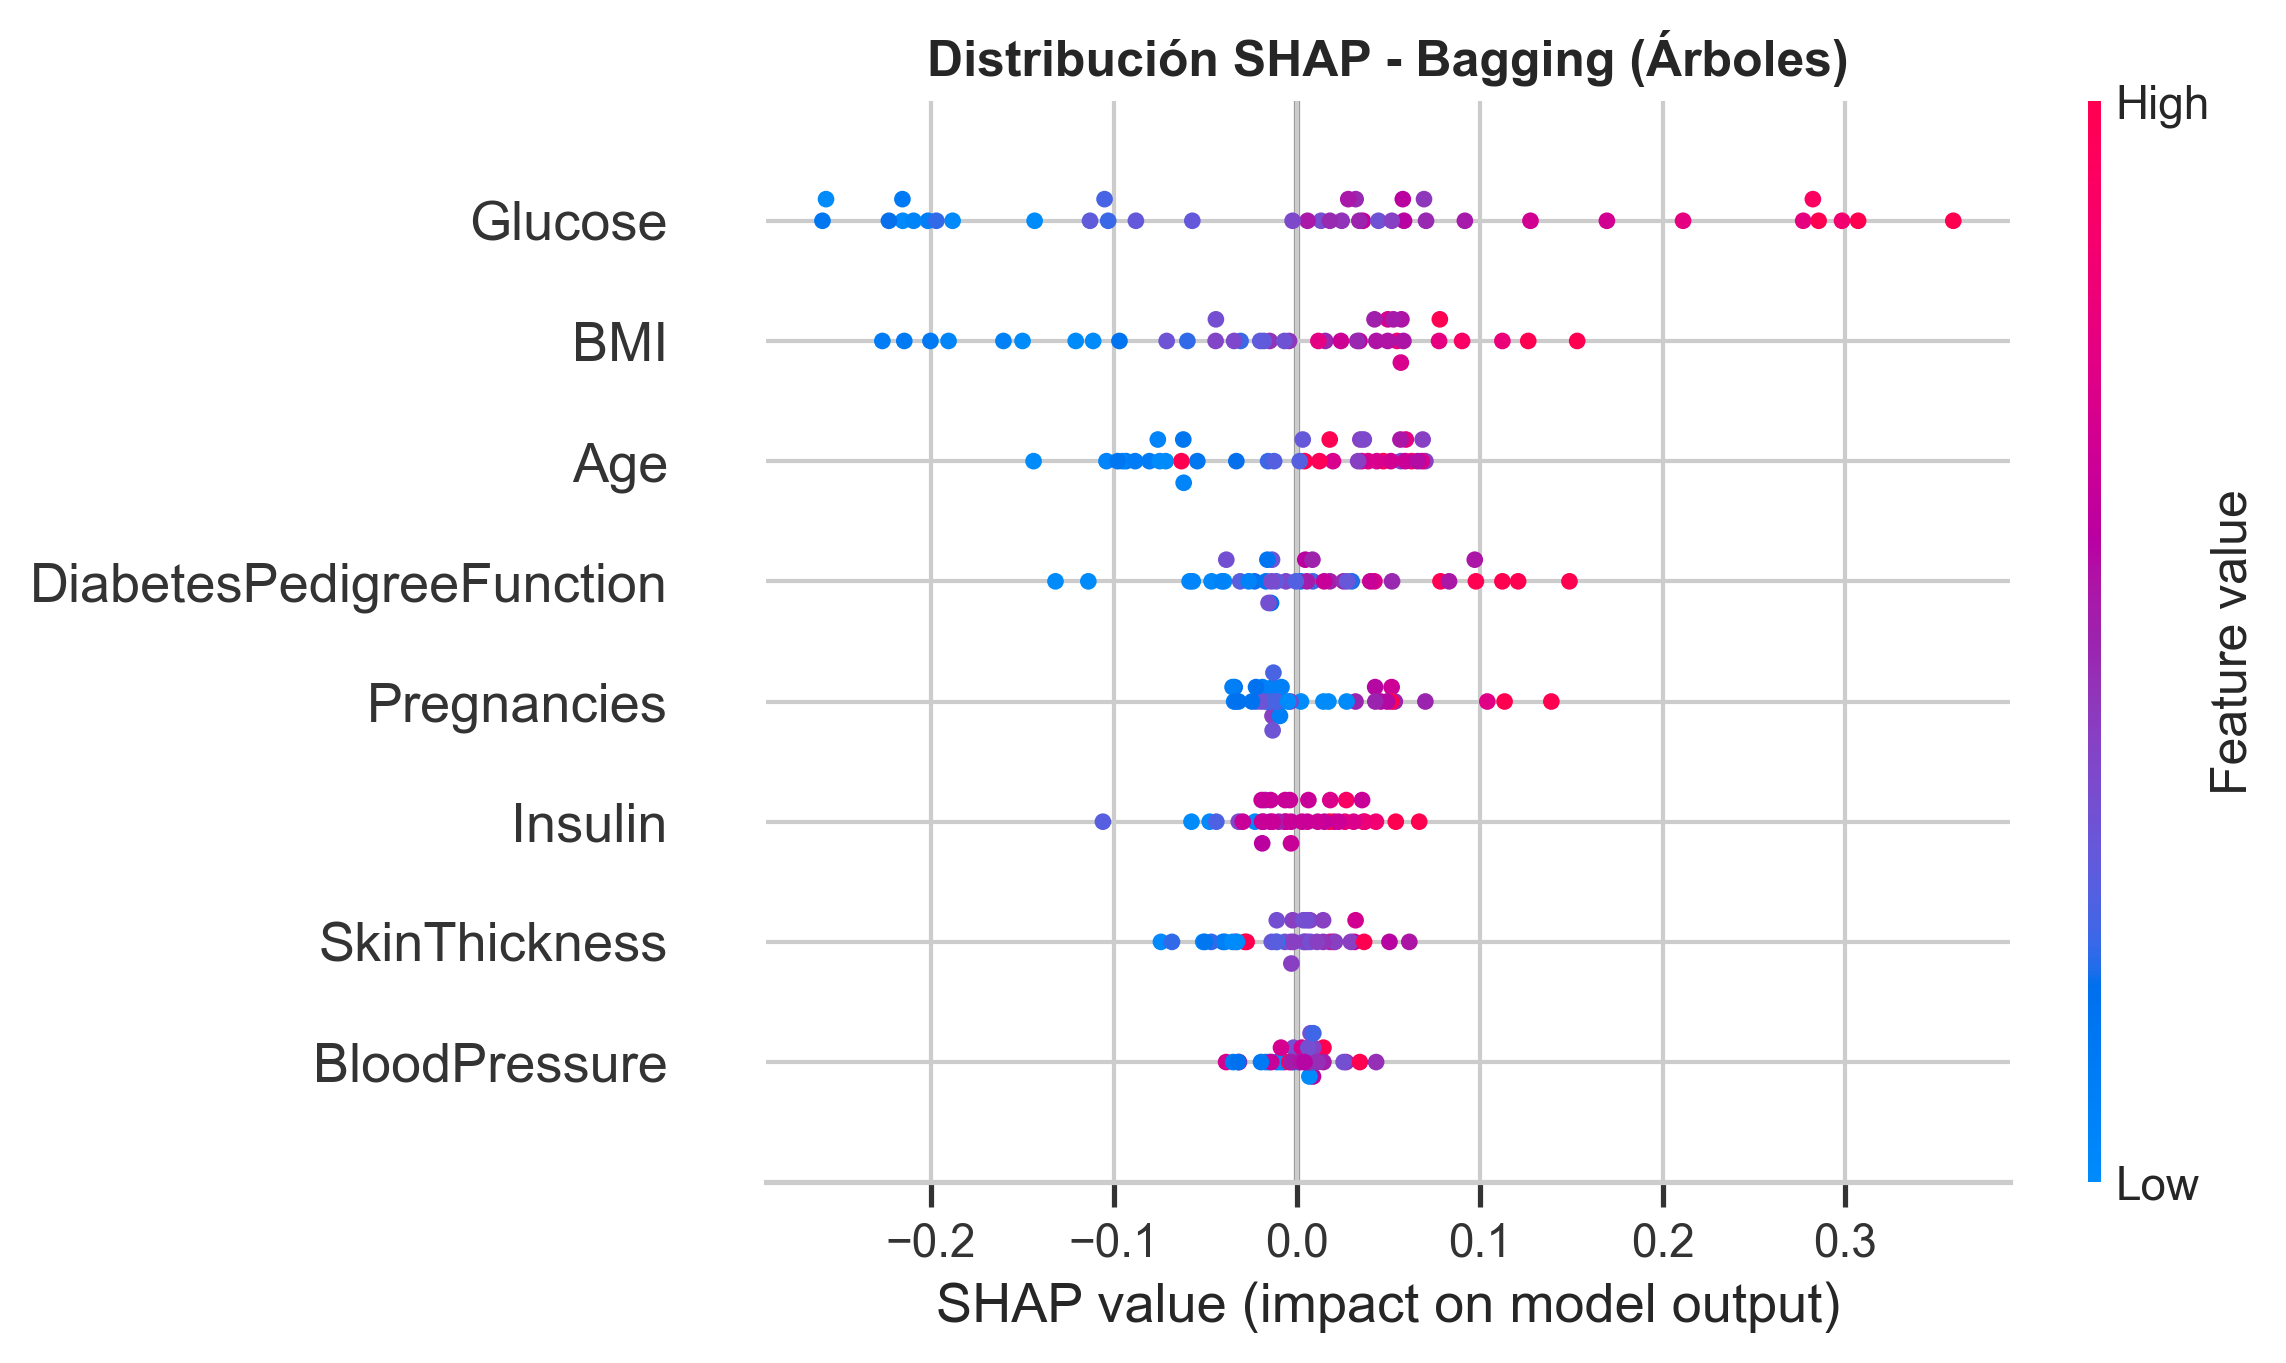
\includegraphics[width=\columnwidth]{22_ganador_beeswarm_shap.png}
  \caption{Distribución SHAP del modelo ganador.}
  \label{fig:shap_beeswarm_bagging}
\end{figure}

\begin{figure}[H]
  \centering
  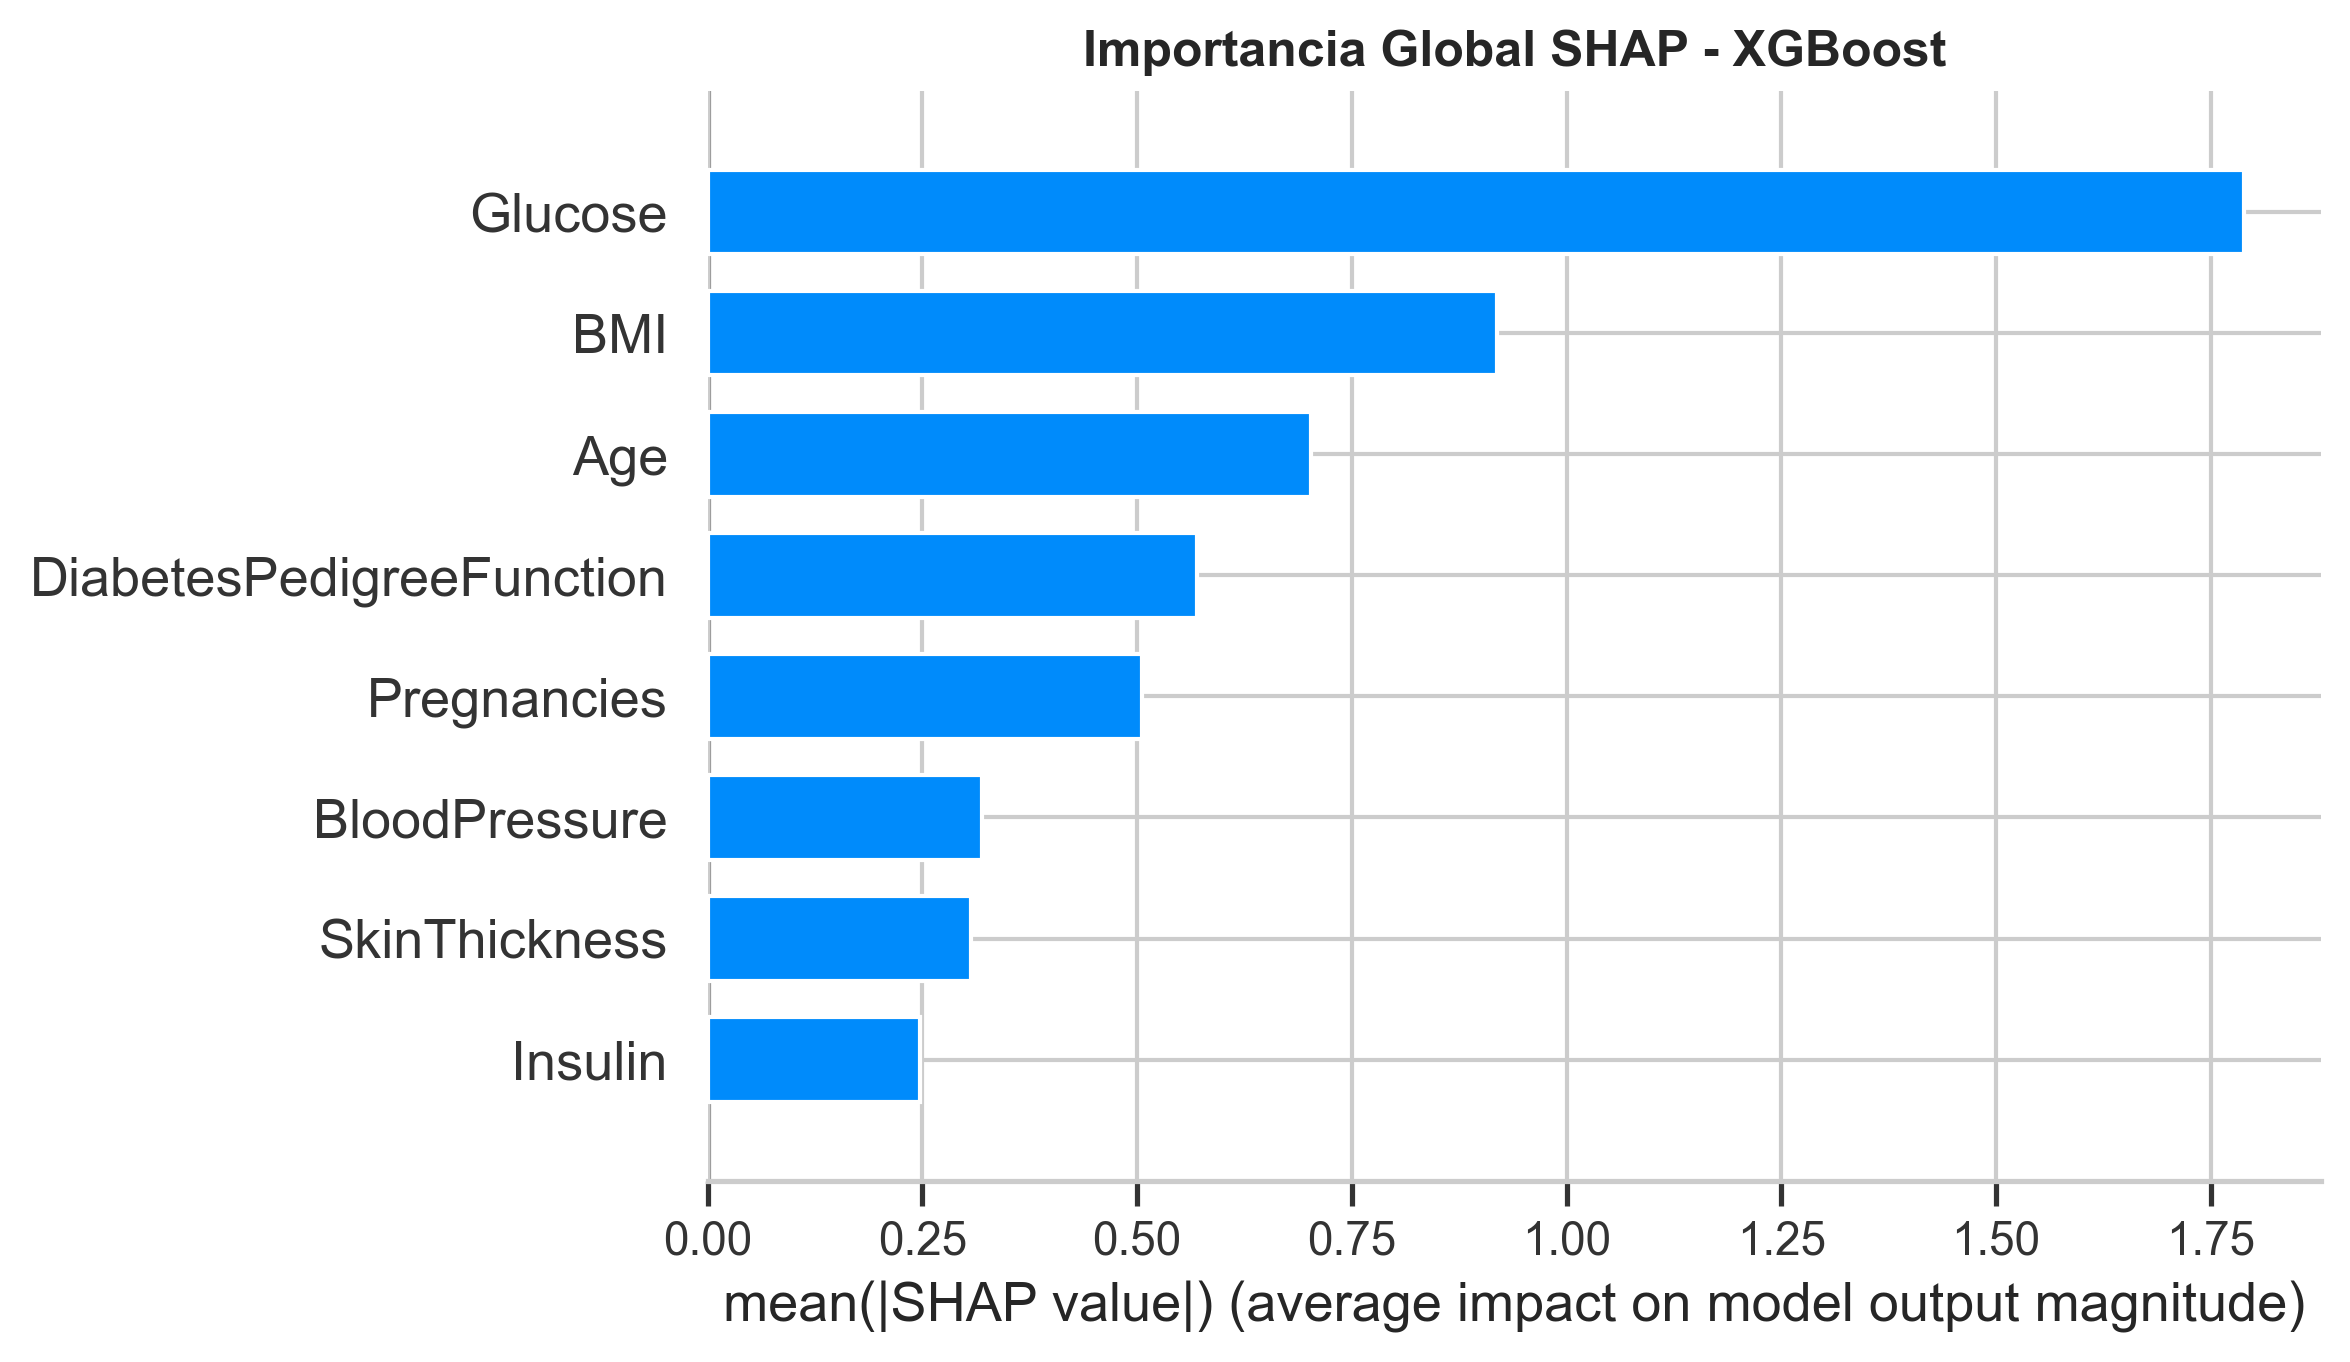
\includegraphics[width=\columnwidth]{23_complemento_arbol_importancia_global_shap.png}
  \caption{Importancia global SHAP complementaria para XGBoost.}
  \label{fig:shap_bar_xgb}
\end{figure}

\textbf{Importancia global (Fig.~\ref{fig:shap_bar_bagging}).} La barra ordena las variables por el promedio del valor absoluto de SHAP, es decir, cuánto mueven la predicción en promedio. \code{Glucose} domina con un impacto medio cercano a $0.14$, casi el doble que \code{BMI} (segunda, $\approx0.076$). Le siguen \code{Age} ($\approx0.054$) y \code{DiabetesPedigreeFunction} ($\approx0.043$), y por debajo \code{Pregnancies}, \code{Insulin}, \code{SkinThickness} y \code{BloodPressure}. Este orden es prácticamente idéntico en el modelo complementario XGBoost (Fig.~\ref{fig:shap_bar_xgb}), lo que indica que la jerarquía de variables no es un artefacto de un modelo concreto, sino una señal robusta de los datos.

\textbf{Dirección del efecto (Fig.~\ref{fig:shap_beeswarm_bagging}).} El gráfico beeswarm añade el sentido de cada contribución: cada punto es un paciente, su posición horizontal es el efecto sobre la probabilidad predicha y el color codifica el valor de la variable (rojo alto, azul bajo). La lectura de las tres variables principales es clínicamente coherente. En \code{Glucose}, los valores altos (rojos) se ubican a la derecha ---suman probabilidad de diabetes--- y los bajos (azules) a la izquierda; la relación es fuerte y prácticamente monótona, con contribuciones que llegan a $+0.35$. En \code{BMI} ocurre lo mismo: mayor índice de masa corporal empuja hacia la clase positiva, consistente con el papel de la obesidad como factor de riesgo. En \code{DiabetesPedigreeFunction}, los valores altos ---mayor carga de antecedentes familiares--- también aportan en dirección positiva. \code{Age} sigue la misma tendencia, aunque con más dispersión alrededor de cero.

\textbf{Contraste con el análisis bivariado.} Un resultado interesante es el de \code{Insulin}: fue el segundo predictor por tamaño de efecto de Mann-Whitney, pero aquí queda entre los de menor aporte. La explicación es que su información está en buena parte contenida en \code{Glucose} ---ambas correlacionan $r=0.68$--- y que su 20\% de faltantes se imputó con la mediana, lo que reduce su varianza útil; el modelo obtiene esa señal principalmente a través de \code{Glucose}, por lo que la contribución \emph{marginal} de \code{Insulin} se diluye. Esto ilustra la diferencia entre la relevancia \emph{individual} de una variable (Mann-Whitney) y su aporte \emph{condicional} dentro de un modelo multivariado (SHAP), y muestra por qué ambos análisis se complementan.

\section{Discusión}

Los resultados muestran que un preprocesamiento cuidadoso ---imputación y límites de winsorizing calculados solo en train, más escalado robusto--- fue tan determinante como la elección del algoritmo, sobre todo para los modelos sensibles a escala y outliers (KNN, SVM, MLP).

El hecho de que Bagging supere ligeramente a XGBoost, LightGBM y Stacking indica que, para este dataset, reducir varianza mediante múltiples árboles bootstrap fue más efectivo que los modelos boosting más complejos. La diferencia con el Stacking es mínima (0.0048 en ROC AUC), por lo que ambos son competitivos; se prefirió Bagging por su mayor ROC AUC y F1 y su menor complejidad operativa. Es esperable, además, que las diferencias tan estrechas entre los modelos del top se estabilicen ---o incluso cambien de orden--- con un volumen de datos mayor, lo que refuerza la idea de que la elección final debe leerse junto con sus limitaciones y no como una ventaja definitiva.

En términos clínicos, el modelo no reemplaza las pruebas diagnósticas. Su valor está en la priorización: ordenar pacientes por riesgo y apoyar circuitos de confirmación con glucemia, HbA1c o prueba de tolerancia oral a la glucosa. Esto dialoga directamente con el contexto peruano descrito, donde una de las brechas principales no es la falta de criterios diagnósticos, sino la heterogeneidad en tiempos, disponibilidad de pruebas y seguimiento.

\subsection{Impacto Esperado en el Circuito de Atención}
\label{sec:impacto}

Como se describió en el contexto peruano, el diagnóstico puede resolverse rápido cuando hay laboratorio disponible, pero el sistema no lo logra de manera homogénea. Las demoras aparecen cuando el paciente no llega en ayunas, cuando debe regresar para una segunda prueba, cuando no hay HbA1c disponible o cuando se pierde continuidad entre resultado anormal y confirmación médica. El modelo puede contribuir en tres puntos:

\begin{enumerate}[leftmargin=1.3em,itemsep=1pt]
  \item \textbf{Triaje tras la medición inicial:} una vez registradas las variables de entrada del paciente ---incluida una medición de glucosa---, usar el score para clasificar a los pacientes en riesgo alto, medio y bajo.
  \item \textbf{Laboratorio:} priorizar HbA1c o glucemia confirmatoria para los pacientes con score alto, reduciendo visitas repetidas.
  \item \textbf{Seguimiento:} generar una lista ordenada de pacientes que no deberían perderse en el circuito de control de crónicos.
\end{enumerate}

\begin{table}[H]
\centering
\caption{Cómo el modelo puede reducir fricciones operativas}
\label{tab:impacto_modelo}
\scriptsize
\begin{tabularx}{\columnwidth}{@{}lX@{}}
\toprule
\textbf{Problema identificado} & \textbf{Uso propuesto del modelo} \\
\midrule
Paciente no llega en ayunas & Si el score es alto, priorizar HbA1c el mismo día cuando esté disponible. \\
Capacidad limitada de consulta & Ordenar pacientes por riesgo para usar cupos rápidos en quienes tienen mayor probabilidad de diabetes. \\
Demora entre resultado y confirmación & Activar circuito corto para scores altos: segunda prueba o cita de confirmación prioritaria. \\
Subregistro y seguimiento débil & Guardar score y predicción como variable de vigilancia para control posterior. \\
Sobrecarga hospitalaria & Derivar casos de menor riesgo a seguimiento programado en primer nivel y acelerar casos de alto riesgo. \\
\bottomrule
\end{tabularx}
\end{table}

En un escenario ideal, el modelo se integraría a una estrategia tipo HEARTS-D en atención primaria: el personal toma variables simples, calcula el score, prioriza confirmación y reduce derivaciones innecesarias al hospital. La reducción no se expresa como ``curar'' la diabetes, sino como disminuir tiempos muertos, mejorar detección oportuna y concentrar recursos en quienes tienen mayor probabilidad de requerir diagnóstico y manejo temprano \cite{ops2024}.

\subsection{Limitaciones}

El estudio presenta varias limitaciones que conviene declarar de forma explícita:

\begin{enumerate}[leftmargin=1.3em,itemsep=1pt]
  \item \textbf{Validez externa.} El modelo se entrenó y evaluó sobre el dataset Pima Indians. El contexto peruano motiva y justifica el problema, pero los resultados no están validados en población peruana; por lo tanto, no debe asumirse transferibilidad directa a establecimientos del país.
  \item \textbf{Preprocesamiento y validación cruzada.} El preprocesamiento se encapsuló en un \code{Pipeline} durante \code{GridSearchCV}, por lo que cada fold recalcula imputación, winsorización, transformación logarítmica y escalado. Aun así, las métricas de CV siguen siendo estimaciones internas del train y no sustituyen la evaluación final en test.
  \item \textbf{Selección del stacking.} El trío de modelos base del stacking se eligió por ROC AUC promedio en validación cruzada sobre train. Esta estrategia evita usar el test para seleccionar los estimadores, aunque el stacking conserva mayor complejidad operativa que el Bagging individual.
  \item \textbf{Coincidencias train-test.} Se detectaron 6 registros idénticos entre train y test y se eliminaron del conjunto de prueba antes de la evaluación final. El test final quedó con 302 observaciones.
  \item \textbf{Discretización por cuantiles.} La discretización de glucosa se realizó con cuantiles (terciles), útil para comparar riesgo relativo, y no con los umbrales clínicos oficiales; por ello, su lectura es exploratoria.
  \item \textbf{Dependencia de la variable de entrada.} El score requiere \code{Glucose} como insumo, de modo que el modelo apoya la priorización de la confirmación y el seguimiento posteriores a una medición inicial, no la decisión de solicitar la primera prueba.
  \item \textbf{Volumen de datos y costo computacional.} El conjunto de entrenamiento (2\,460 registros) es modesto y las diferencias entre los mejores modelos son estrechas. Un mayor volumen daría estimaciones de desempeño más estables y evaluaciones más confiables, pero a costa de mayores tiempos de entrenamiento y de búsqueda de hiperparámetros; escalar el enfoque exigiría acotar la rejilla o paralelizar el cómputo.
\end{enumerate}

\section{Conclusiones}

\begin{itemize}[leftmargin=1.3em,itemsep=2pt]
  \item \textbf{Mejor modelo.} El ganador global fue Bagging de árboles (ROC AUC 0.8937, F1 0.7222, accuracy 0.8344), por delante del Stacking Top-3 (0.8889) y de la Regresión Logística, mejor modelo base (0.8822). El buen desempeño de esta última muestra que una frontera lineal regularizada sigue siendo competitiva en datos clínicos tabulares.
  \item \textbf{Variable determinante.} \code{Glucose} es el predictor dominante, con evidencia convergente de cuatro análisis independientes ---EDA, Mann-Whitney U, tasa de diabetes por tercil y SHAP---, y con una dirección coherente: a mayor glucosa, mayor riesgo estimado.
  \item \textbf{Rigor del flujo.} El pipeline controla la fuga de información: se retiraron las coincidencias train--test y todo el preprocesamiento se recalcula dentro de cada fold de la validación cruzada.
  \item \textbf{Uso aplicado.} El valor del modelo está en priorizar riesgo ---ordenar pacientes para acelerar confirmación (HbA1c, glucemia o PTOG) y seguimiento en atención primaria--- y no en diagnosticar de forma autónoma.
  \item \textbf{Alcance.} Los resultados no están validados en población peruana y las diferencias entre los mejores modelos son estrechas; su consolidación requiere mayor volumen de datos y validación local.
\end{itemize}

\section{Trabajo Futuro}

El trabajo futuro se organiza en tres frentes que van de lo más urgente a lo más aplicado. El primero es la \textbf{validez externa}, condición para cualquier uso real: validar el modelo con datos locales peruanos, evaluar su equidad (\emph{fairness}) por edad y región, y monitorear su estabilidad en el tiempo, ya que un modelo entrenado en otra población tiende a degradarse al cambiar de contexto. El segundo frente busca \textbf{enriquecer y afinar el modelo}: incorporar variables de laboratorio como HbA1c o glucosa en ayunas cuando estén disponibles, calibrar las probabilidades con métodos como Platt o \emph{isotonic regression} ---de modo que el score pueda leerse como una probabilidad real y no solo como un ordenamiento--- y fijar el umbral de decisión según el costo clínico de los falsos positivos y negativos. El tercer frente es la \textbf{puesta en uso}: convertir el artefacto exportado \code{mejor\_modelo\_diabetes.pkl} en una herramienta simple de inferencia que reciba los datos de un paciente y devuelva su score de priorización, cerrando el ciclo entre el análisis y la práctica clínica.

\section*{Agradecimientos}

Los autores agradecen a la Universidad ESAN y al curso de Minería de Datos por el marco académico para el desarrollo del proyecto. Asimismo, se reconoce el uso del dataset Pima Indians Diabetes y de fuentes públicas nacionales para contextualizar la problemática de diabetes en el Perú.

\begin{thebibliography}{00}

\bibitem{idf2021}
International Diabetes Federation, \textit{IDF Diabetes Atlas}, 10th ed., Brussels: IDF, 2021.

\bibitem{who2021}
World Health Organization, ``Diabetes,'' WHO, 2021. \url{https://www.who.int/news-room/fact-sheets/detail/diabetes}

\bibitem{kaggle}
E. Aboelnaga, ``Diabetes Dataset,'' Kaggle, 2023. \url{https://www.kaggle.com/datasets/ehababoelnaga/diabetes-dataset}

\bibitem{kavakiotis2017}
I. Kavakiotis et al., ``Machine Learning and Data Mining Methods in Diabetes Research,'' \textit{Computational and Structural Biotechnology Journal}, vol. 15, pp. 104--116, 2017.

\bibitem{sisodia2018}
D. Sisodia and D. S. Sisodia, ``Prediction of Diabetes Using Classification Algorithms,'' \textit{Procedia Computer Science}, vol. 132, pp. 1578--1585, 2018.

\bibitem{chen2016}
T. Chen and C. Guestrin, ``XGBoost: A Scalable Tree Boosting System,'' in \textit{Proc. 22nd ACM SIGKDD}, pp. 785--794, 2016.

\bibitem{ke2017}
G. Ke et al., ``LightGBM: A Highly Efficient Gradient Boosting Decision Tree,'' in \textit{NeurIPS}, vol. 30, 2017.

\bibitem{lundberg2017}
S. M. Lundberg and S.-I. Lee, ``A Unified Approach to Interpreting Model Predictions,'' in \textit{NeurIPS}, vol. 30, 2017.

\bibitem{minsa2024}
Ministerio de Salud del Perú, ``La diabetes se constituye como séptima causa de muerte en nuestro país,'' MINSA, 2024.

\bibitem{inei2023}
Instituto Nacional de Estadística e Informática, \textit{Perú: Enfermedades No Transmisibles y Transmisibles, 2023}, INEI, 2024.

\bibitem{ops2024}
Organización Panamericana de la Salud, ``HEARTS en Perú: hacia una mejor atención de la diabetes en el primer nivel,'' OPS/OMS, 2024.

\bibitem{cdc2024}
Centro Nacional de Epidemiología, Prevención y Control de Enfermedades, ``Actualización en vigilancia de diabetes: casos registrados enero 2023--junio 2024,'' CDC Perú, 2024.

\bibitem{cdc2025}
Centro Nacional de Epidemiología, Prevención y Control de Enfermedades, ``Sala situacional de diabetes: red notificante nacional,'' CDC Perú, actualización 2025.

\bibitem{pp0018}
Ministerio de Salud del Perú, ``Programa Presupuestal 0018: enfermedades no transmisibles, reportes de diabetes,'' MINSA, 2023--2025.

\bibitem{inei_adulto_mayor}
Instituto Nacional de Estadística e Informática, ``Situación de la población adulta mayor,'' INEI, 2025.

\bibitem{multilab_glucosa}
Multilab, ``Ficha de examen: glucosa basal y postprandial,'' Laboratorio clínico, 2024--2026.

\bibitem{multilab_hba1c}
Multilab, ``Hemoglobina glicosilada HbA1c: información y tiempos de entrega,'' Laboratorio clínico, 2024--2026.

\bibitem{loayza2025}
Hospital Nacional Arzobispo Loayza, ``Solicitar exámenes de laboratorio: tiempos de entrega de exámenes generales,'' Gobierno del Perú, 2025.

\bibitem{box2015}
G. E. P. Box, G. M. Jenkins, G. C. Reinsel, and G. M. Ljung, \textit{Time Series Analysis: Forecasting and Control}, 5th ed. Hoboken, NJ, USA: Wiley, 2015.

\bibitem{hyndman2021}
R. J. Hyndman and G. Athanasopoulos, \textit{Forecasting: Principles and Practice}, 3rd ed. Melbourne, Australia: OTexts, 2021. \url{https://otexts.com/fpp3/}

\bibitem{bcrpdata}
Banco Central de Reserva del Perú, ``BCRPData: series estadísticas mensuales PN01765AM, PN01723AM y PN01652XM,'' BCRP, 2026. \url{https://estadisticas.bcrp.gob.pe}

\bibitem{igp_icen}
Instituto Geofísico del Perú, ``Índice Costero El Niño (ICEN),'' IGP/ENFEN, 2026. \url{http://met.igp.gob.pe/datos/ICEN.txt}

\bibitem{takahashi2015}
K. Takahashi, \textit{Boletín Técnico: Generación de modelos climáticos para el pronóstico de la ocurrencia del Fenómeno El Niño}, vol. 2, no. 3. Lima, Perú: Instituto Geofísico del Perú, 2015. \url{https://repositorio.igp.gob.pe/bitstreams/11a1226e-4f5a-4990-97fa-c4be061da3fc/download}

\bibitem{inei2017}
Instituto Nacional de Estadística e Informática, ``Producción Nacional: marzo 2017,'' Informe Técnico N.\textdegree{} 05, INEI, Lima, 2017. \url{https://www.inei.gob.pe/media/MenuRecursivo/boletines/05-informe-tecnico-n05_produccion-nacional-mar2017.pdf}

\bibitem{bcrp_moneda198}
Banco Central de Reserva del Perú, ``El vínculo entre minería, energía e industria en el Perú,'' \textit{Revista Moneda}, no. 198. \url{https://www.bcrp.gob.pe/docs/Publicaciones/Revista-Moneda/moneda-198/moneda-198-13.pdf}

\bibitem{dickey1979}
D. A. Dickey and W. A. Fuller, ``Distribution of the estimators for autoregressive time series with a unit root,'' \textit{Journal of the American Statistical Association}, vol. 74, no. 366, pp. 427--431, 1979.

\bibitem{kpss1992}
D. Kwiatkowski, P. C. B. Phillips, P. Schmidt, and Y. Shin, ``Testing the null hypothesis of stationarity against the alternative of a unit root,'' \textit{Journal of Econometrics}, vol. 54, no. 1--3, pp. 159--178, 1992.

\bibitem{ljungbox1978}
G. M. Ljung and G. E. P. Box, ``On a measure of lack of fit in time series models,'' \textit{Biometrika}, vol. 65, no. 2, pp. 297--303, 1978.

\bibitem{taylor2018}
S. J. Taylor and B. Letham, ``Forecasting at scale,'' \textit{The American Statistician}, vol. 72, no. 1, pp. 37--45, 2018.

\bibitem{hyndman2006}
R. J. Hyndman and A. B. Koehler, ``Another look at measures of forecast accuracy,'' \textit{International Journal of Forecasting}, vol. 22, no. 4, pp. 679--688, 2006.

\bibitem{theil1966}
H. Theil, \textit{Applied Economic Forecasting}. Amsterdam, The Netherlands: North-Holland, 1966.

\bibitem{diebold1995}
F. X. Diebold and R. S. Mariano, ``Comparing predictive accuracy,'' \textit{Journal of Business \& Economic Statistics}, vol. 13, no. 3, pp. 253--263, 1995.

\bibitem{engle1982}
R. F. Engle, ``Autoregressive conditional heteroscedasticity with estimates of the variance of United Kingdom inflation,'' \textit{Econometrica}, vol. 50, no. 4, pp. 987--1007, 1982.

\bibitem{jarque1980}
C. M. Jarque and A. K. Bera, ``Efficient tests for normality, homoscedasticity and serial independence of regression residuals,'' \textit{Economics Letters}, vol. 6, no. 3, pp. 255--259, 1980.

\bibitem{prokhorenkova2018}
L. Prokhorenkova, G. Gusev, A. Vorobev, A. V. Dorogush, and A. Gulin, ``CatBoost: Unbiased boosting with categorical features,'' in \textit{NeurIPS}, vol. 31, 2018.

\bibitem{ledell2020}
E. LeDell and S. Poirier, ``H2O AutoML: Scalable automatic machine learning,'' in \textit{Proc. 7th ICML Workshop on Automated Machine Learning (AutoML)}, 2020.

\bibitem{hochreiter1997}
S. Hochreiter and J. Schmidhuber, ``Long short-term memory,'' \textit{Neural Computation}, vol. 9, no. 8, pp. 1735--1780, 1997.

\bibitem{cho2014}
K. Cho et al., ``Learning phrase representations using RNN encoder-decoder for statistical machine translation,'' in \textit{Proc. EMNLP}, pp. 1724--1734, 2014.

\bibitem{schuster1997}
M. Schuster and K. K. Paliwal, ``Bidirectional recurrent neural networks,'' \textit{IEEE Transactions on Signal Processing}, vol. 45, no. 11, pp. 2673--2681, 1997.

\bibitem{vaswani2017}
A. Vaswani et al., ``Attention is all you need,'' in \textit{NeurIPS}, vol. 30, pp. 5998--6008, 2017.

\bibitem{nie2023}
Y. Nie, N. H. Nguyen, P. Sinthong, and J. Kalagnanam, ``A time series is worth 64 words: Long-term forecasting with Transformers,'' in \textit{Proc. ICLR}, 2023.

\bibitem{liu2008}
F. T. Liu, K. M. Ting, and Z.-H. Zhou, ``Isolation forest,'' in \textit{Proc. 8th IEEE International Conference on Data Mining (ICDM)}, pp. 413--422, 2008.

\bibitem{das2024}
A. Das, W. Kong, R. Sen, and Y. Zhou, ``A decoder-only foundation model for time-series forecasting,'' in \textit{Proc. 41st International Conference on Machine Learning (ICML)}, PMLR, vol. 235, 2024.

\bibitem{timesfm3}
Google Research, ``TimesFM 3.0 (PyTorch),'' model card, Hugging Face, 2026. \url{https://huggingface.co/google/timesfm-3.0-pytorch}

\bibitem{patchtstfm}
IBM Research, ``Granite TimeSeries PatchTST-FM-r2,'' model card, Hugging Face, 2026. \url{https://huggingface.co/ibm-granite/granite-timeseries-patchtst-fm-r2}

\bibitem{toto2026}
E. Khwaja et al., ``Toto 2.0: Time series forecasting enters the scaling era,'' arXiv:2605.20119 [cs.LG], 2026. doi: 10.48550/arXiv.2605.20119

\end{thebibliography}

\end{document}